\chapter{Methodology}
\label{chap:Research methods}

Taking into account the research questions posed in \autoref{sec:research questions} and the research gaps identified in \autoref{sec:research gaps}, this chapter presents a detailed narrative of the steps taken to develop and implement the \ac{KRL-based BCF}. For better understanding, this methodology is broken down into 2 core steps.

\begin{enumerate}
    \item 
    \textbf{\acf{LBD} modeling}: This section walks through a prototypical data modeling example to delineate the technical aspects and key considerations for building an effective \ac{BIM-KG} for training \ac{KRL} models. Although a building automation use case is used, the same steps can be used for other domains such as heritage, quantity-takeoff and energy analysis. 

    \item 
    \textbf{Performance analysis of \ac{KRL} on \ac{LBD}}: This section explores the integration of \ac{KRL} with \ac{LBD} (\acp{BIM-KG}), focusing on the use of performance analysis experiments whose goal is not to identify the best \ac{KRL} model configurations, but rather examine more closely how model performance can be affected by modifications to the training step, selection of hyperparameters, their optimization and initialization approaches and data set split mechanics.
\end{enumerate}

The experimental results from step 2 are used to define the prerequisites for integrating \ac{KRL} with \acp{BIM-KG} in a domain-independent framework. Again, although a building automation use case is used to formulate the framework, it is extensible to other \ac{AEC/FM} domains and a prototype will be presented to illustrate such extensions while assessing the feasibility and applicability of the framework.

\begin{figure}[!th]
    \centering
    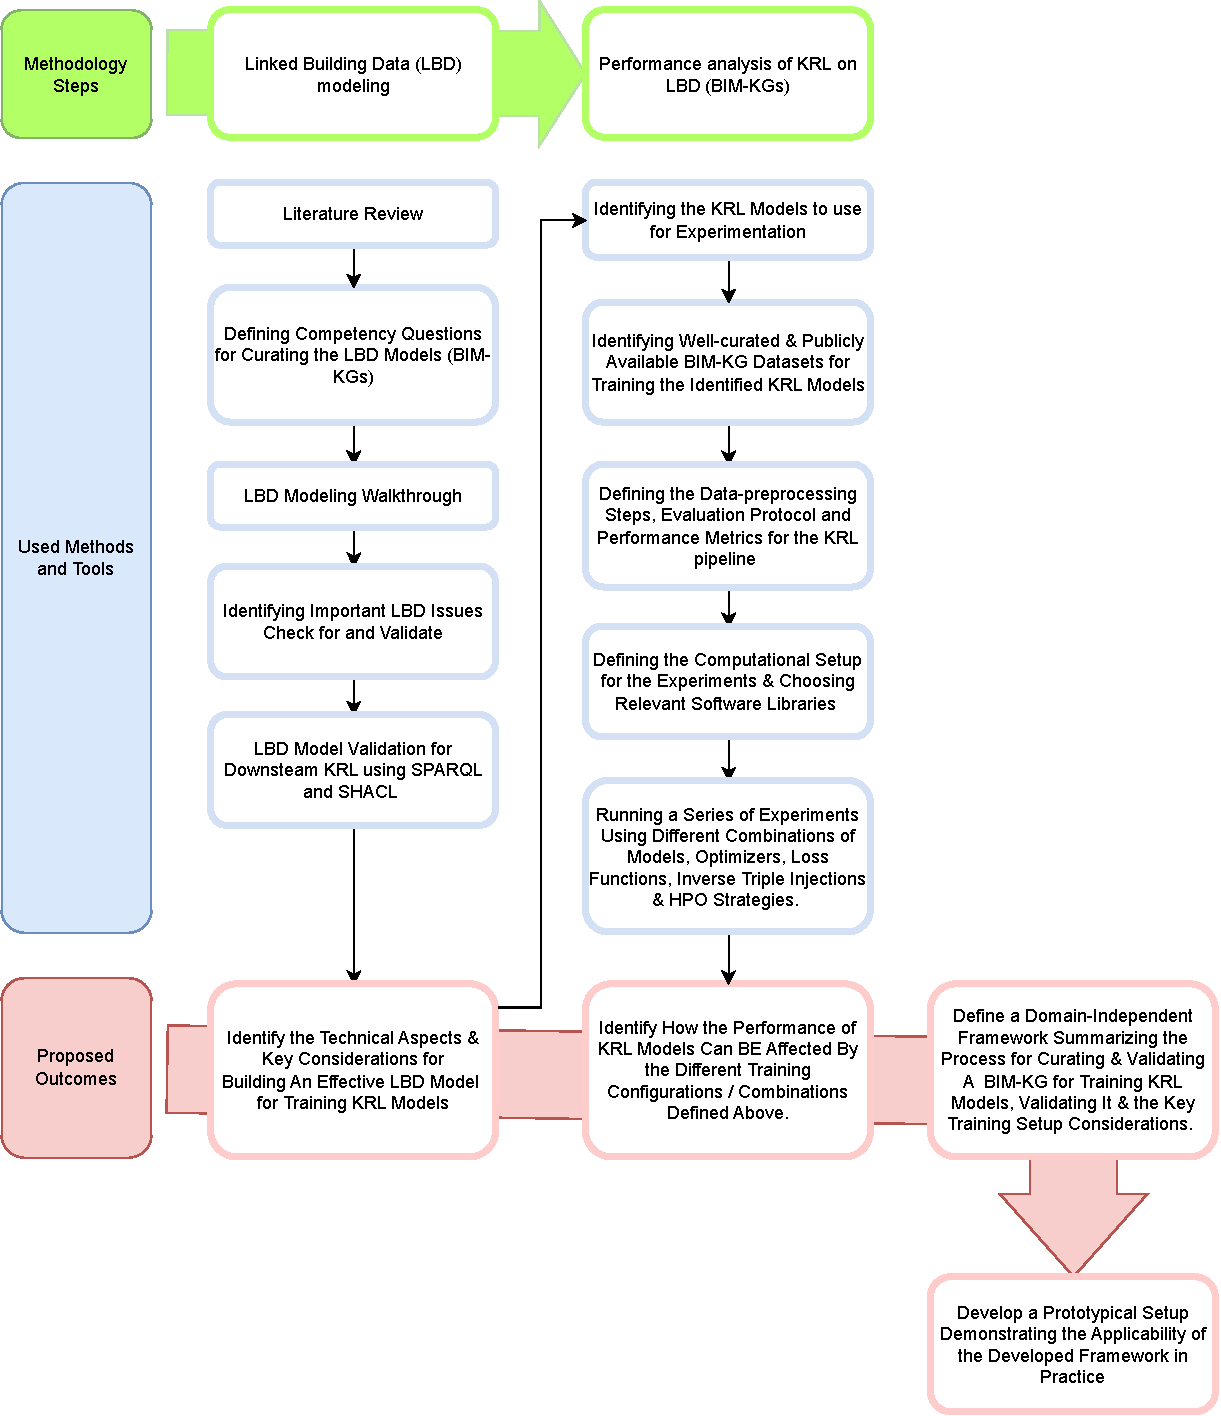
\includegraphics[width=1.0\textwidth]{figures/Methodology.pdf}
    \caption{The research methodology overview} \label{fig: research methodology overview}
\end{figure}

\section{\acf{LBD} Modeling}\label{sec: linked building data modeling}
This work adopts domain-agnostic \acp{SWT} to demonstrate the process of developing a \ac{BIM-KG} within the building automation domain while using carefully crafted competency questions to scope the specific objectives that the \ac{BIM-KG} needs to satisfy.

\subsection{Competency Questions as an \ac{LBD} Modeling Guide}

Rather than develop new data modelling vocabularies (ontologies), this work adopts existing vocabularies from the \ac{LBDCG} \citep{W3C-LinkedDataCommunityGroup2018}. A specific ontology of interest is the ifcOWL ontology \citep{Pauwels2016}. As per the \ac{IFC}4 Add2 release\footnote{\url{https://standards.buildingsmart.org/IFC/DEV/IFC4/ADD2_TC1/OWL/index.html}}, ifcOWL has about 770 classes,
approximately 1190 object properties, and around 60 datatype properties. This granularity
is one of ifcOWL’s main strengths, offering a level of detail that surpasses many other
\ac{BIM} ontologies. It caters to a wide array of applications from architectural design to facility management. However, this granularity can pose challenges, as the numerous classes and properties, along with their complex relationships, can become unwieldy for certain smaller use cases. Additionally, there is a risk of
higher computational demands for querying and inference, potentially hindering performance
in real-time building automation tasks applications. Given this, smaller and more focused ontologies, some branching off ifcOWL need to be adopted. Throughout this section, precise competency questions are crafted to guide the choice of modular ontologies and to help maintain focus on the objectives that the curated \ac{LBD} model (\ac{BIM-KG}) has to fulfil.

\begin{enumerate}
\item 
\textbf{Competency Question 1 (CQ1)}: \textit{How to semantically describe the high-level concepts of a building in a way that formulates a semantic extension baseline for describing low-level building information relevant for indoor environment monitoring and control?}

 To answer this question, the \acf{BOT}\footnote{https://w3c-lbd-cg.github.io/bot/} \citep{Rasmussen2017} is employed as it is deemed appropriate for encoding relationships between the main components of a building (site, building, storey and space) using a highly modular and simplistic set of semantic blocks. In \ac{BOT}, a building consists of zones in a hierarchy. The subclass of a zone is a site which contains a building(s), storey(s), and a space(s). A zone can be adjacent to another zone or even contain other zones. It can also be bounded by physical building elements or even contain them. Building elements can also host other elements (a wall hosting a sensor). \Autoref{BOT classes} summarizes the classes adopted from \ac{BOT} while \autoref{BOTBuilding} provides an intuitive description of how \ac{BOT} is used to describe a site, \texttt{<UNM>}, having a building, \texttt{<Block\_B>}, containing a storey, \texttt{<Floor\_3>} with a certain space, \texttt{<Office\_204>}.
 \begin{figure}[b]
    \centering
    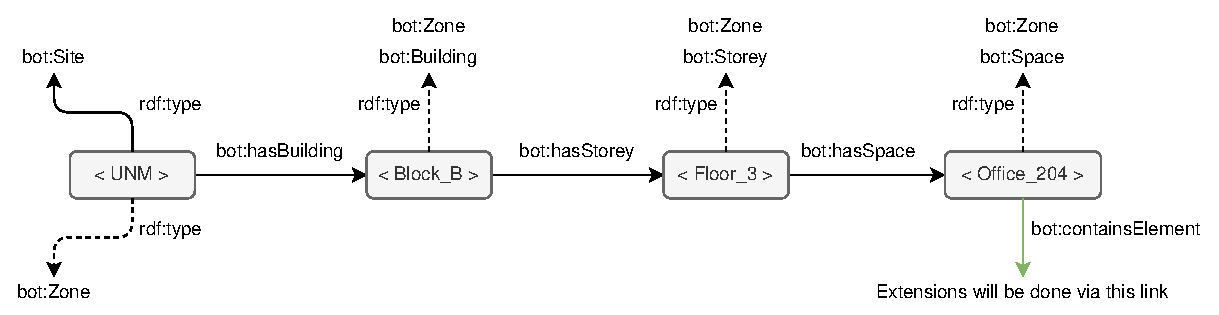
\includegraphics[width=1.0\textwidth]{figures/BOT.eps}
    \caption{Using BOT classes and properties to describe the high level semantic topological details of a building} \label{BOTBuilding}
\end{figure}
\begin{table}[t]
	\centering
 \caption{BOT classes and properties to be adopted}
	\begin{tabular}{l|l|l}
		\hline \hline
		Classes (domain) & Properties & Classes(range) \bigstrut \\ \hline
		\texttt{bot:Zone} & \texttt{bot:containsZone} & \texttt{bot:Zone} \bigstrut \\
		& \texttt{bot:adjascentZone} & \texttt{bot:Zone} \bigstrut \\
		\texttt{bot:Site} & \texttt{bot:hasBuilding} & \texttt{bot:Building} \bigstrut \\
		\texttt{bot:Building} & \texttt{bot:hasStorey} & \texttt{bot:Storey} \bigstrut \\
		\texttt{bot:Storey} & \texttt{bot:hasSpace} & \texttt{bot:Space} \bigstrut \\
		\texttt{bot:Space} & \texttt{bot:containsElement} & \texttt{bot:Element} \bigstrut \\
		\texttt{bot:Element} & \texttt{bot:hostsElement} & \texttt{bot:Element} \bigstrut \\
	\end{tabular}
	
	\label{BOT classes}
\end{table}
 The respective entity connections are made via the object properties; \texttt{bot:hasBuilding}, \texttt{bot:hasStorey} and \texttt{bot:hasSpace}. Explicitly asserted relationships/properties are shown by the solid line arrows while those that are automatically inferred are shown by the dotted line arrows. The back-end inference rules at play here, are defined in \ac{BOT} via the ranges and domains summarized in \autoref{BOT classes}). A corresponding machine-readable serialization (Turtle format) of the data model (\ac{BIM-KG}) is shown in \autoref{lst:BOTbuildingttl}. With a \ac{BOT} foundation, semantic extensions can be made to describe low-level details about specific features of interest contained in the space, \texttt{<Office\_204>} such as sensors and walls via another object property, \texttt{bot:containsElement} as the extension point.   


    
\begin{lstlisting}[language=N3, caption={Turtle serialization of the information modelled in figure above}, label=lst:BOTbuildingttl]
@prefix rdf: <http://www.w3.org/1999/02/22-rdf-syntax-ns#> .
@prefix bot: <https://w3id.org/bot#> .

# Site location (UNM) for some building of interest (Block_B)
<UNM> a bot:Site ;
  bot:hasBuilding <Block_B> .

# Block_B has some storey of interest Floor_3
<Block_B> bot:hasStorey <Floor_3> .

# Floor_3 has some space(zone) of interest Office_204
<Floor_3> bot:hasSpace <Office_204> .
\end{lstlisting}

\item 
\textbf{Competency Question 2 (CQ2)}: \textit{How to semantically describe a feature of interest within an indoor space while encoding its measurable properties, corresponding property values and property states in a way that allows tracking changes, deletions and revisions?}

For this question, the \acf{SSN}\footnote{https://www.w3.org/TR/vocab-ssn/} \citep{Haller2017} ontology is adopted. At its core, exists a lightweight but self-contained ontology \ac{SOSA} encapsulating elementary classes necessary for the semantic description of features of interest and their properties, sensor observations, and feature sampling procedures to describe tractable sensor observations and actuation behaviour. Furthermore, the \ac{SEAS} \citep{Lefrancois2016} ontology is used to avail semantic extensions to \ac{SSN}. \ac{SEAS} is an ecosystem of modules that together, provide semantic vocabulary to describe physical systems and their interrelations. Among these, is the \texttt{seas:FeatureOfInterestOntology}\footnote{https://w3id.org/seas/FeatureOfInterestOntology} for describing features of interest and their properties and the \texttt{seas:EvaluationOntology}\footnote{https://w3id.org/seas/EvaluationOntology} for describing evaluations of these properties. However, these natively have no semantics to encode property states in a way that can be tracked over time. For this, the \ac{OPM}\footnote{https://w3c-lbd-cg.github.io/opm/} \citep{Rasmussen2018a} is deemed relevant. The specific classes and properties it provides for this work are summarized in \autoref{OPM}. To illustrate the usage of these ontologies to answer competency question 2, a direct semantic extension is made to the \texttt{bot:Space}, \texttt{<Office\_204>}. First, it is defined as a \texttt{sosa:FeatureOfInterest} having two measurable properties; \texttt{<Office\_204\#temperature>} and \texttt{<Office\_204\#humidity>}, both defined via the relation \texttt{ssn:hasProperty}. To stay complaint with OPM and satisfy competency question 2, both properties are required to have atleast one \texttt{opm:hasPropertyState} relation for assigning states to the properties. A property state in \ac{OPM} is an evaluation that contains the value and metadata of a property deemed true at a specific point in time. \ac{OPM} also specifies that as a minimum, a property state should have a value and preferably, a generation time, an assignment that can respectively be done via the properties; \texttt{schema:value}, from \url{schema.org}\footnote{https://schema.org/value} and \texttt{prov:generatedAtTime}, from the Provenance Ontology\footnote{https://www.w3.org/TR/prov-o/}. \texttt{<Office\_204>} is further defined to have two elements which are both walls. One wall, \texttt{<Office\_204/east>}, is located on the eastern side of the room and the other wall, \texttt{<Office\_204/south>}, on the southern side. Each of them is described as both a \texttt{sosa:FeatureOfInterest} and a \texttt{sosa:Platform}. The latter simply means that each of the walls hosts another entity, in this case, a \texttt{<NodeMCU>} \ac{PCB} that is also a \texttt{sosa:Platform} hosting a DHT22 temperature and humidity sensor. Because the temperature and humidity properties are defined on the \texttt{<Office\_204>} entity, but are implicitly being measured from the interior walls \texttt{<Office\_204/east>} and \texttt{<Office\_204/south>} via the embedded sensors, it is necessary to describe each wall as a \texttt{sosa:Sample}\footnote{https://www.w3.org/TR/vocab-ssn/\#SOSASample}. A more intuitive graphical description of this data modelling process is provided in figure \ref{SSN_OPM_SEAS} together with its Turtle serialization in \autoref{lst:SSN_OPM_SEASttl}. Another ontology that can be adopted for explicit definition of complex functionality of smart appliances and their controllability, is \ac{SAREF}\footnote{https://saref.etsi.org/} \citep{Daniele2015}. The starting point of the \ac{SAREF} vocabulary is a device. Currently, much of the semantic vocabulary for describing device controllability has been availed by the \ac{SEAS}, \ac{SSN} \ac{SOSA} and \ac{BOT} however, should the need arise for more explicit descriptions of systems and their energy consumption behaviour, \ac{SAREF} extensions can be adopted.  
\begin{table}[!h]
	\centering
        \caption{SEAS classes and properties adopted for this work's data model}
	\begin{tabular}{l|l}
		\hline \hline
		Classes & Properties  \bigstrut \\ \hline
		\texttt{seas:ElectricPowerSystem} & \texttt{seas:isPoweredBy}  \bigstrut \\
		\texttt{seas:TemperatureEvaluation} & \texttt{seas:optimizes}  \bigstrut \\
		\texttt{seas:AgentComfortEvaluation} & \texttt{seas:thermalTransmittance}  \bigstrut \\
		\texttt{seas:MaximumComfortableEvaluation} & \texttt{seas:relativeToAgent} \bigstrut \\
		\texttt{seas:MinimumComfortableEvaluation} & \texttt{seas:evaluatedSimpleValue} \bigstrut \\
		\texttt{seas:Battery} & \texttt{seas:hasTemporalContext} \bigstrut \\
	\end{tabular}
	\label{SEAS}
\end{table}

\begin{table}[!h]
	\centering
        \caption{OPM classes and properties adopted for this work's data model}
	\begin{tabular}{l|l}
		\hline \hline
		Classes & Properties  \bigstrut \\ \hline
		\texttt{opm:Assumed} & \texttt{opm:hasPropertyState}  \bigstrut \\
		\texttt{opm:CurrentPropertyState} & \bigstrut \\
		\texttt{opm:PropertyState} & \bigstrut \\
		\texttt{opm:Confirmed} & \bigstrut \\
		\texttt{opm:OutdatedPropertyState} & \bigstrut \\
		\texttt{opm:Deleted} & \bigstrut \\
		
	\end{tabular}
	\label{OPM}
\end{table}
\end{enumerate}

\begin{lstlisting}[language=N3, caption={Turtle serialization of the information modelled in figure \ref{SSN_OPM_SEAS}.}, label=lst:SSN_OPM_SEASttl]
@prefix rdf: <http://www.w3.org/1999/02/22-rdf-syntax-ns#> .
@prefix bot: <https://w3id.org/bot#> .
@prefix xsd:  <http://www.w3.org/2001/XMLSchema#> .
@prefix cdt:   <http://w3id.org/lindt/custom_datatypes#> .
@prefix schema: <http://schema.org/>.
@prefix sosa: <http://www.w3.org/ns/sosa/> .
@prefix ssn: <http://www.w3.org/ns/ssn/> .
@prefix seas: <https://w3id.org/seas/> .
@prefix opm: <https://w3id.org/opm#> .
@prefix prov:  <http://www.w3.org/ns/prov#> .

# Office_204 (FOI) hosts some 2 walls at the east and south that will host 
# some sensors. The space also has two properties temperature and humidity
<Office_204> a sosa:FeatureOfInterest ;
  bot:containsElement <Office_204/east>, <Office_204/south> ;
  ssn:hasProperty <Office_204#temperature> , <Office_204#humidity> .

# Office_204 east side wall to host a NodeMCU board with 
# a DHT22 temp and  hum sensor.  
<Office_204/east> a sosa:FeatureOfInterest , sosa:Sample , sosa:Platform ;
  sosa:hosts <NodeMCU_1> .
  
# Office_204 south side wall to host a NodeMCU board with a DHT22 temp and 
# hum sensor.                
<Office_204/south> a sosa:FeatureOfInterest , sosa:Sample , sosa:Platform ;
  sosa:hosts <NodeMCU_2> ;

# DESCRIPTION OF PCB BOARDS HOSTING THE SENSORS
##############################################################

# NodeMCU 1 board hosted by the office_204 east side wall.
<NodeMCU_1> a ssn:System , sosa:Platform ;
  sosa:hosts <DHT22/01> ;
  ssn:hasSubSystem <DHT22/01> .

# NodeMCU 2 board hosted by the office_204 south side wall.
<NodeMCU_2> a ssn:System , sosa:Platform ;
  sosa:hosts <DHT22/02> ;
  ssn:hasSubSystem <DHT22/02> .
  
# Assigning a state to the temperature property of Office #204   
<Office_204#temperature> 
  opm:hasPropertyState <Office_204#temperature_state_48906948_er8t78> .
  
# Assigning semantics to Office_204#temperature_state_48906948_er8t78 state
<Office_204#temperature_state_48906948_er8t78> 
  a opm:Confirmed , 
    opm:CurrentPropertyState ;
  schema:value "30.5 Cel"^^cdt:temperature ;
  prov:generatedAtTime "2020-07-28T16:41:17.711+02:00"^^xsd:dateTime.

# Assigning a state to the humidity property of Office #204  
<Office_204#humidity> 
  opm:hasPropertyState <Office_204#humidity_state_40039548_gktiy8> .
  
# Assigning semantics to Office_204#humidity_state_40039548_gktiy8 state
<Office_204#humidity_state_40039548_gktiy8> 
  a opm:Confirmed , 
    opm:CurrentPropertyState ;
  schema:value "85.0 %"^^cdt:ucum ;
  prov:generatedAtTime "2020-07-28T16:41:17.711+02:00"^^xsd:dateTime. 
\end{lstlisting}

\begin{figure}[htbp]
    \centering
    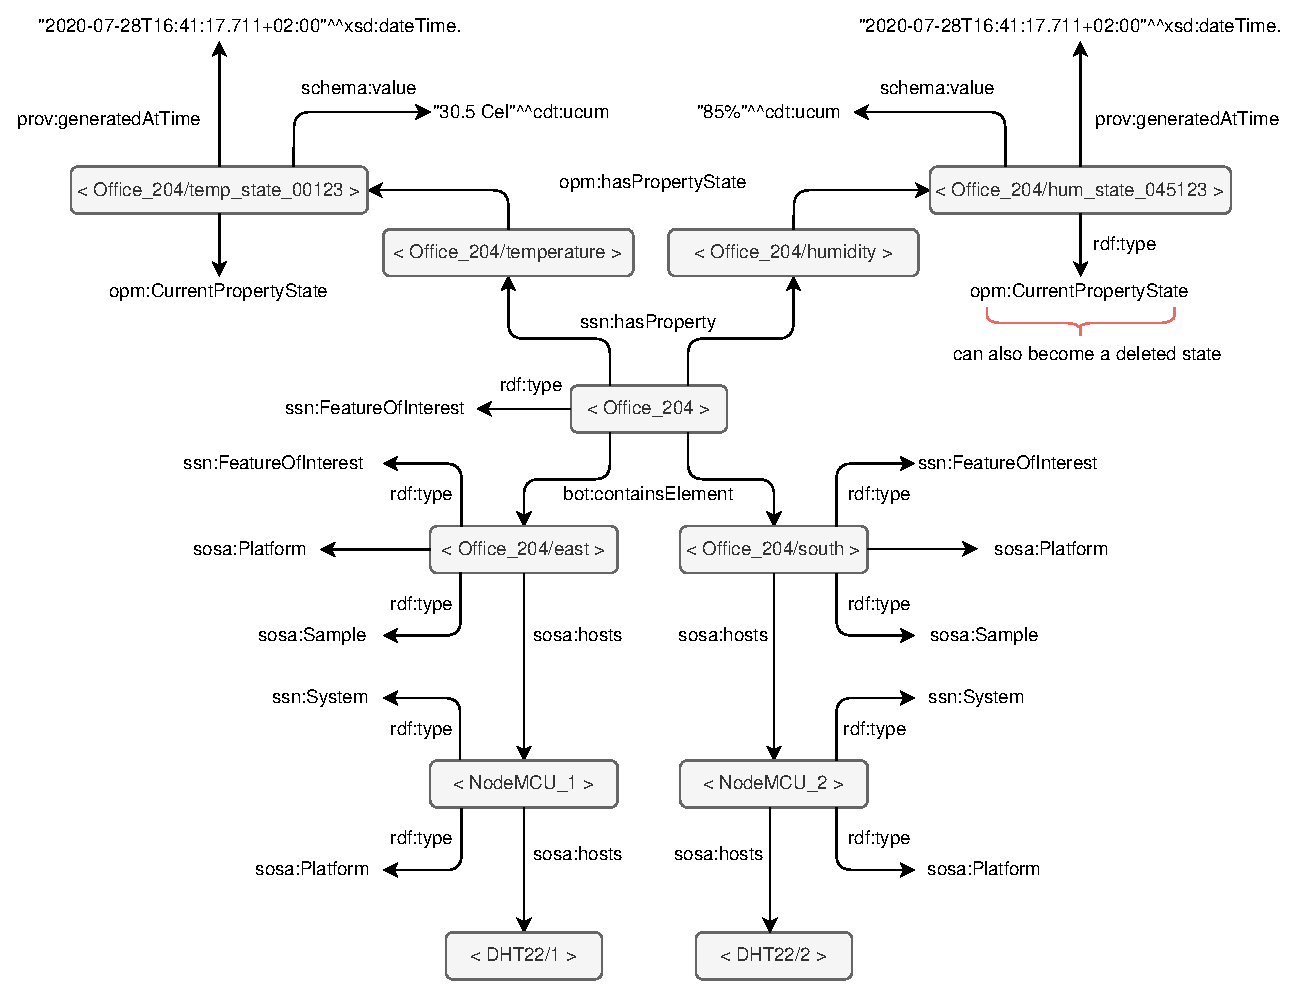
\includegraphics[width=1\textwidth]{figures/SSN_OPM_SEAS.eps}
    \caption{Using SSN/SOSA, OPM and SEAS ontologies to extend the semantic details of a building to encapsulate indoor zone information about sensors, elements contained within, their properties and state management ( simplistic view).} \label{SSN_OPM_SEAS}
\end{figure}

Below is a summary of the modular ontologies that have been adopted to solve the competency questions above;
\begin{enumerate}
    \item 
    \textbf{\acf{BOT}\footnote{https://w3c-lbd-cg.github.io/bot/}}: \ac{BOT} \citep{Rasmussen2017} provides the foundation vocabulary necessary to model the core topological aspects of a building such as a site, a building, a storey, a space, and an element in a space. \ac{BOT} is chosen for its simplicity, modularity and extensibility.

    \item 
    \textbf{\acf{SSN}\footnote{https://www.w3.org/TR/vocab-ssn/} and \acf{SOSA}}: \ac{SSN} and its lightweight version \ac{SOSA} \citep{Haller2017} offer the vocabulary necessary to describe sensors and their observations.

    \item
    \textbf{\ac{SEAS}}: \ac{SEAS} \citep{Lefrancois2016} offers an ontology to describe smart appliances and their communication with the grid.

    \item 
    \textbf{\ac{OPM}}: \ac{OPM} \citep{Rasmussen2018a} provides a schema for describing temporal properties that are subject to changes as the building design evolves.

    \item 
    \textbf{SAREF (Smart Appliances REFerence)}: The \ac{SAREF} \citep{Daniele2015} suite of ontologies is a set of standardized frameworks designed to ensure that different \ac{IoT} solutions from various providers can work together seamlessly.
\end{enumerate}

\subsection{\ac{LBD} Model Validation for downstream \ac{KRL}}
The continued standardization of Semantic Web approaches in the \ac{AEC/FM} industry has resulted in an unprecedented volume of building data being included on the web as Linked Data. Although gathering and publishing such massive amounts of data is certainly a step in the right direction for the industry, the effectiveness of this data hinges on its quality. In other words, simply having access to an extensive web of building data does not guarantee valuable insights or improved decision-making. Within the context of \ac{KRL}, the potency of a model is tightly bound to the quality of its input data (knowledge graph). Factors such as data integrity, consistency, density, noise level, completeness, redundancy, and structural regularities in a knowledge graph can significantly influence the quality of what the model learns (the resultant embeddings), which in the case of \ac{FM}, potentially affects a building's operational behavior. From a data engineering perspective, data quality is often defined as its fitness for use within a certain domain, use case, or application. From a data engineering perspective, data quality is defined by its suitability for specific domains, use cases, or applications. Even datasets with quality issues can hold value if they meet the standards required for particular applications. For instance, the web contains content of varying quality but is still widely regarded as highly useful. Even datasets with quality issues can be valuable if they meet the required standards for particular applications. For example, while the web contains content of varying quality, it remains highly regarded for its usefulness. In the AEC/FM industry, most data-intensive applications rely on some form of data-fitness guidelines that specify the fundamental requirements input data must satisfy to be deemed useful. Interestingly, there is little consensus on what a good data-fitness guideline is. Each guideline tends to target a specific subset of needs with some rules even introduced by personal preference; others are meant to prevent very specific types of data errors from earlier efforts within an organization. Perhaps the most dooming aspect of many of the guidelines is that they rarely allow for comprehensive tool-based data compliance checks. Tool-based checks are important for reviewing hundreds of thousands of data points (triples) in large enterprise knowledge graphs. To be effective though, I will argue that the set of rules has to be small in the beginning. Such a small set, of course, cannot be all-encompassing, but it can give us a foothold to achieve measurable effects on data reliability and verifiability. 

In this research, focusing on structural consistency, data completeness, and redundancy serves as a pragmatic starting point to tackle the most immediate threats to data reliability and minimize cascading errors further along the KRL pipeline. \textit{Structural consistency} guarantees that the \ac{BIM-KG} adheres to its predefined schema and semantic constraints, ensuring that the underlying representation is reliable for parsing, processing and analysis. \textit{Data completeness} verifies that all essential information for a specific usecase is present. \textit{Redundancy checking} helps prevent duplication and conflicting data, which can otherwise obscure important insights or lead to erroneous conclusions. Although these three issues do not cover every possible aspect of data quality, they lay a strong foundation for the development of more nuanced or domain-specific data-fitness guidelines in the industry.

This research uses \ac{SHACL}\footnote{https://www.w3.org/TR/shacl/} to illustrate the procedures for validating a \ac{BIM-KG} against specific quality criteria. Simultaneously, \ac{SPARQL}\footnote{https://www.w3.org/TR/sparql11-query/} is employed for its data extraction and manipulation capabilities, facilitating cleanup and transformation tasks on the \ac{BIM-KG} whenever issues are identified. It is important to note that SPARQL can also be used for validation due to its high expressivity. Before detailing the validation process, a brief narrative of the chosen \ac{BIM-KG} issues to check for is provided below. 

\begin{enumerate}
    \item 
    \textbf{Structural Consistency}: Because \ac{KRL} relies on message-passing, any structural irregularities in the \ac{BIM-KG} can disrupt the learning process and impact the quality of the resulting embeddings. Irregularities can arise from inconsistent or incomplete data entry in the underlying \ac{BIM} model. For example, if a \ac{BIM-KG} contains the following triples: 
    \texttt{<Office\_204>} $\xrightarrow{\text{bot:containsElement}}$ \texttt{<NodeMCU\_1>}, \texttt{<Building\_UNM>} $\xrightarrow{\text{bot:hasSpace}}$ \texttt{<Office\_204>},
    \texttt{<Building\_UNM>} $\xrightarrow{\text{bot:hasSpace}}$ \texttt{<Office\_204>}, \texttt{<Building\_UNM>} $\xrightarrow{\text{bot:hasSpace}}$ \texttt{<NodeMCU\_1>}, the inferred knowledge `\texttt{<Building\_UNM>} $\xrightarrow{\text{bot:containsElement}}$ \texttt{<NodeMCU\_1>}' contradicts the logical expression of the third triple. Using \ac{SHACL}, specific constraints can be defined to dictate the acceptable configurations for nodes and relationships in the \ac{BIM-KG}. In addition, \ac{SPARQL} can be leveraged to query the \ac{BIM-KG} and identify any deviations from the enforced \ac{SHACL} shapes and corrective actions are taken using \ac{SPARQL}'s \ac{CRUD} operations.

    \begin{figure}
        \centering
        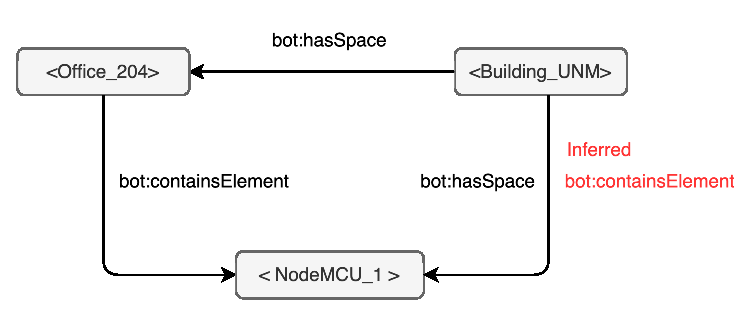
\includegraphics[width=0.8\textwidth]{figures/inconsistent-kg.eps}
        \caption{Example of inconsistent knowledge in a \ac{BIM-KG}} \label{INCONSISTENT-KG}
    \end{figure}

    \item 
    \textbf{Data Completeness}: In the context of this thesis, data completeness refers to how well a \ac{BIM-KG} covers the relevant domain knowledge i.e., the proportion of existing data to the total data required for a specific problem. Data completeness is a multi-faceted problem encompassing several dimensions such as accuracy, timeliness, relevancy, objectivity, and believability etc. What constitutes `complete' data can vary depending on the application or use case, meaning that different situations may have different requirements for what makes data complete. For an indoor environment control task, the instance \texttt{<Office\_204>} might suffer from a data completeness problem if its measurable properties, \texttt{<Office\_204\#temperature>} and \texttt{<Office\_204\#humidity>}, are absent in the \ac{BIM-KG}, whereas this would not be of concern for a cost estimation use case.  When a \ac{KRL} model is trained on such incomplete data, its resultant embeddings miss out on potentially important contextual information, leading to inaccurate downstream inferences and analyses. \cite{Zaveri2016QualitySurvey} reviewed several quality assessment approaches for Linked Data and categorized knowledge graph completeness into four classes: schema completeness, property completeness, population completeness and inter-linking completeness. This thesis does not go into the details of these classes, however, \cite{Zaveri2016QualitySurvey}'s work, is a starting point for other researchers in the \ac{AEC/FM} domain to investigate data completeness issues that are specific to \acp{BIM-KG}.

    \item 
    \textbf{Redundancy}: Redundancy occurs when multiple nodes in a \ac{BIM-KG} hold the same type of information but are labeled with different names or identifiers. A hypothetical example with intentional redundancy would be a particular space, say \texttt{<Office\_204>}, being represented by two different properties in the same dataset, such as \texttt{http://example.org/spaceID} and \texttt{http://example.org/name}. This redundancy (\texttt{spaceID} and \texttt{name} ) can ideally be solved by merging the two properties and keeping only one unique identifier. Property or entity duplication in a \ac{BIM-KG} can misguide a \ac{KRL} model's message-passing process resulting in malformed embeddings.
\end{enumerate}

\noindent To illustrate the validation process for the \ac{BIM-KG} discussed in \autoref{sec: linked building data modeling}, the requirements below are utilized. It is important to note that these requirements are typically defined by a domain expert for a specific use case. 

\begin{enumerate}
    \item 
    Every \texttt{sosa:FeatureOfInterest} has to host at least one \texttt{ssn:System}.

    \item 
    Every \texttt{ssn:System} has to host at least one \texttt{sosa:Sensor}.

    \item 
    Every \texttt{ssn:Property} has to have an associated \texttt{opm:PropertyState}.

    \item 
    Every \texttt{opm:CurrentPropertyState} has a defined value (\texttt{schema:value}) and a timestamp (\texttt{prov:generatedAtTime}).
\end{enumerate}
 
\noindent To check these conditions, validations that are rooted in \ac{SPARQL} and \ac{SHACL} are adopted. First, \ac{SPARQL} \texttt{ASK} queries are provided for each condition, which return either true if the condition is violated, or false if the data meets the condition (see \autoref{lst:validation1} - \autoref{lst:validation4}):

\begin{enumerate}
\item 
\texttt{sosa:FeatureOfInterest} hosts at least one \texttt{ssn:System}:

\begin{lstlisting}[language=N3, caption={This query returns true if there exists at least one \texttt{sosa:FeatureOfInterest} that does not host any \texttt{ssn:System}.}, label=lst:validation1]
PREFIX ssn: <http://www.w3.org/ns/ssn/>.
PREFIX sosa: <http://www.w3.org/ns/sosa/>.

ASK WHERE {
  ?foi a sosa:FeatureOfInterest .
  FILTER NOT EXISTS { 
      ?foi sosa:hosts ?system . 
      ?system a ssn:System . 
  }
}
\end{lstlisting}

\item 
Every \texttt{ssn:System} hosts at least one sensor:
\begin{lstlisting}[language=N3, caption={This query returns \texttt{true} if there exists at least one \texttt{ssn:System} that does not host any \texttt{sosa:sensor}}, label=lst:validation2]
PREFIX ssn: <http://www.w3.org/ns/ssn/>.
PREFIX sosa: <http://www.w3.org/ns/sosa/>.

ASK WHERE {
  ?system a ssn:System .
  FILTER NOT EXISTS {
    ?system sosa:hosts ?sensor
    ?sensor a sosa:Sensor
  }
}
\end{lstlisting}

\item 
Every \texttt{ssn:Property} has an associated state:
\begin{lstlisting}[language=N3, caption={This query returns \texttt{true} if there exists at least one \texttt{ssn:Property} that has no property state}, label=lst:validation3]
PREFIX ssn: <http://www.w3.org/ns/ssn/>.
PREFIX sosa: <http://www.w3.org/ns/sosa/>.
PREFIX opm: <https://w3id.org/opm#>.

ASK WHERE {
  ?property a ssn:Property .
  FILTER NOT EXISTS {
    ?property opm:hasPropertyState ?state
  }
}

\end{lstlisting}

\item 
Every \texttt{opm:CurrentPropertyState} has a defined value and a timestamp:
\begin{lstlisting}[language=N3, caption={This query returns \texttt{true} if there exists at least one \texttt{opm:CurrentPropertyState} that does not have either a \texttt{schema:value} or \texttt{prov:generatedAtTime} property.}, label=lst:validation4]
PREFIX opm: <https://w3id.org/opm#>.
PREFIX schema: <http://schema.org/>.
PREFIX prov:  <http://www.w3.org/ns/prov#>.

ASK WHERE {
  ?state a opm:CurrentPropertyState .
  FILTER NOT EXISTS { ?state schema:value ?value }
  FILTER NOT EXISTS { ?state prov:generatedAtTime ?time }
}
\end{lstlisting}

\end{enumerate}

\noindent \ac{SHACL} is more expressive and capable of defining more complex constraints than \ac{SPARQL} alone as shown in \autoref{lst:shacl} below.

\begin{lstlisting}[language=N3, caption={\ac{SHACL} shapes to express the same constraints defined in listings \ref{lst:validation1} - \ref{lst:validation4}}, label=lst:shacl]
@prefix sh: <http://www.w3.org/ns/shacl#> .
@prefix xsd:  <http://www.w3.org/2001/XMLSchema#> .
@prefix schema: <http://schema.org/>.
@prefix sosa: <http://www.w3.org/ns/sosa/> .
@prefix ssn: <http://www.w3.org/ns/ssn/> .
@prefix opm: <https://w3id.org/opm#> .

# Shape for FeatureOfInterest
:FeatureOfInterestShape
    a sh:NodeShape ;
    sh:targetClass sosa:FeatureOfInterest ;
    sh:property [
        sh:path sosa:hosts ;
        sh:class ssn:System ;
        sh:minCount 1 ;
        sh:message "A FeatureOfInterest must host at least one System."
    ] .

# Shape for System
:SystemShape
    a sh:NodeShape ;
    sh:targetClass ssn:System ;
    sh:property [
        sh:path sosa:hosts ;
        sh:minCount 1 ;
        sh:message "A System must host at least one sensor."
    ] .

# Shape for Property
:PropertyShape
    a sh:NodeShape ;
    sh:targetClass ssn:Property ;
    sh:property [
        sh:path opm:hasPropertyState ;
        sh:minCount 1 ;
        sh:message "A Property must have an associated state."
    ] .

# Shape for CurrentPropertyState
:CurrentPropertyStateShape
    a sh:NodeShape ;
    sh:targetClass opm:CurrentPropertyState ;
    sh:property [
        sh:path schema:value ;
        sh:minCount 1 ;
        sh:message "A CurrentPropertyState must have a defined value."
    ] ;
    sh:property [
        sh:path prov:generatedAtTime ;
        sh:datatype xsd:dateTime ;
        sh:minCount 1 ;
        sh:message "A CurrentPropertyState must have a timestamp."
    ] .

\end{lstlisting}

\noindent In the above \ac{SHACL} shapes graph, each \texttt{sh:NodeShape} defines the shape for a specific class of nodes, e.g., \texttt{sosa:FeatureOfInterest}, \texttt{ssn:System}, \texttt{ssn:Property}, and \texttt{opm:CurrentPropertyState}. For each shape, \texttt{ sh:property} is used to specify constraints for the properties of the nodes that conform to the shape.
For instance, in \texttt{:FeatureOfInterestShape}, the \texttt{sh:property} construct requires that each \texttt{sosa:FeatureOfInterest} must host (\texttt{sosa:hosts}) at least one (\texttt{sh:minCount 1}) \texttt{ssn:System}. Similarly, \texttt{:SystemShape} specifies that each \texttt{ssn:System} must host at least one sensor. The \texttt{sh:message} constructs are used to provide human-readable error messages that are displayed when a constraint is violated. In practice, \ac{SHACL} validation is performed using \texttt{pySHACL}\footnote{https://github.com/RDFLib/pySHACL}, a Python library developed by \texttt{RDFlib}\footnote{https://github.com/RDFLib/rdflib}. The high-level implementation details for this are shown in \autoref{lst:rdf-and-shapes-loading}.

\begin{lstlisting}[language=python, caption={Python script for loading \ac{RDF} data and \ac{SHACL} shapes for validating a knowledge graph}, label=lst:rdf-and-shapes-loading]
import rdflib
from pyshacl import validate

# Load RDF Data
data_graph = rdflib.Graph()
data_graph.parse("path_to_the_kg_data", format='turtle')

# Load SHACL Shapes
shapes_graph = rdflib.Graph()
shapes_graph.parse("path_to_your_shacl_shapes", format='turtle')

# Run the validation
val = validate(data_graph, shacl_graph=shapes_graph)
conforms, results_graph, results_text = val

# Check if the data passed the SHACL validation
if conforms:
    print("The data graph passed SHACL validation!")
else:
    print("The data graph failed SHACL validation.")
    print(results_text)

\end{lstlisting}

\subsection{Conclusion}
This section provided a prototypical example for building a \ac{BIM-KG} for training \ac{KRL} models. Several existing \ac{AEC/FM} vocabularies (ontologies) were used instead of introducing new ones, a workflow that is strongly encouraged. Two approaches were presented to maintain the focus of the \ac{BIM-KG}'s scope to the task at hand: crafting competency questions as a proactive approach and using \texttt{SHACL} and \ac{SPARQL} for \ac{BIM-KG} validation as a reactive approach. To ensure that the modelled \ac{BIM-KG} is sufficient in the \ac{KRL} phase, a pragmatic starting point is taken by considering three issues as important to check for: structural consistency, data completeness and redundancy. Arguably these tackle the most immediate threats to data reliability and minimize cascading errors further along the KRL pipeline while laying a strong foundation for other researchers to develop of more nuanced or domain-specific data-fitness guidelines in the industry.

\section{Performance Analysis of \acf{KRL} on \acf{LBD}}\label{sec: relational-learning}
% For \ac{KRL} to impact the \ac{AEC/FM} domain, this research emphasizes the critical importance of comprehensively reporting \ac{KRL} model architectures, training setups, hyperparameters, and dataset splits to enhance trust, reproducibility and understanding of \ac{KRL}-based methods among \ac{AEC/FM} stakeholders and researchers. 


The section develops and formalizes a methodology for applying \ac{KRL} to \acp{BIM-KG} using performance analysis experiments. An overview of the models, datasets, and evaluation protocol used for the experiments is discuused herein.

\subsection{Models}
Several \ac{KRL} models have been introduced in \autoref{KRL models}, differentiated primarily by their score functions. For this research's experiments, five \ac{KRL} models were chosen: ComplEx, DistMult, RotatE, TransE and TransH. One key motivation for focusing on these baseline models lies in the relatively nascent intersection of \ac{KRL} and \acp{BIM-KG}. While deep learning approaches are undoubtedly state-of-the-art in many other domains, the maturity of KRL applications in the \ac{AEC/FM} field (particularly involving \acp{BIM-KG}) is still in its infancy. Employing advanced neural architectures prematurely risks overshadowing or missing the fundamental considerations vital to establishing a stable methodological foundation. As a result, this research prioritizes a controlled exploration of well-established KRL models—namely ComplEx, DistMult, RotatE, TransE, and TransH—that have proven effective on widely used benchmark datasets in knowledge graph literature. 

Another reason is that these baseline models are easier to interpret and less resource-intensive to implement and tune, making them suitable for a domain that has not yet standardized on key aspects of \ac{KRL} best practices. By demonstrating how these simpler, yet robust approaches perform on \acp{BIM-KG}, this work aims to distill essential insights—such as the impact of data quality, hyperparameter selection, and training procedures—that might otherwise be obscured by the greater complexity and heavier computational requirements of deep neural network models. Once these basic principles are clarified and validated, future research will be better equipped to evaluate whether advanced neural architectures offer a practical advantage for this domain—or whether their additional complexity complicates adoption without providing commensurate gains.



% These models are well-regarded baseline techniques from the existing literature, cover a wide range of methodologies, and have been extensively investigated in the context of drug discovery \citep{Paliwal2020PreclinicalGraphs, Zheng2021PharmKG:Mining}, whose data structures closely mirror those of \acp{BIM-KG}.  
In this work, all models consume  triples sampled from the 2 publicly available \acp{BIM-KG} datasets\footnote{\url{https://github.com/BIM-and-Automation-Laboratory/phd-source/tree/main/hpo-study/datasets}} described in \autoref{subsec:experimental_datasets}.
The internal structure and outputs of each model are discussed below.
\begin{enumerate}
    \item 
    \textbf{TransE} is one of the earliest and most influential \ac{KRL} models for link prediction. It embeds both entities and relations from a knowledge graph into a low-dimensional vector space, typically $\mathbb{R}^d$, and represents relationships as translation vectors. As illustrated in \autoref{transe-illustration}, the core intuition is that for a triple $(h, r, t)$, where $h$ is the \emph{head} entity, $r$ is the \emph{relation}, and $t$ is the \emph{tail} entity, the embedding of $h$ plus the embedding of $r$ should be close to the embedding of $t$ (\autoref{eq:transE_intuition}):

\begin{equation}
\label{eq:transE_intuition}
    \mathbf{h} + \mathbf{r} \approx \mathbf{t}
\end{equation}

\begin{figure}[t]
        \centering      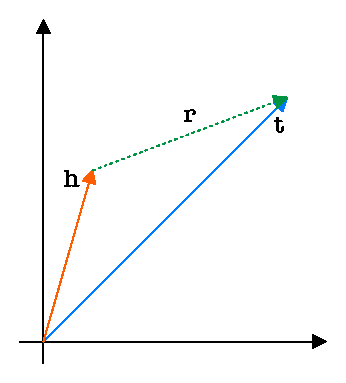
\includegraphics[width=0.5\textwidth]{figures/transe_illustration.pdf}
        \caption{A simple illustration of TransE} \label{transe-illustration}
\end{figure}

where $\mathbf{h}, \mathbf{t} \in \mathbb{R}^d$ are the entity embeddings, and $\mathbf{r} \in \mathbb{R}^d$ is the relation embedding. During training, each triple is presented along with a negatively corrupted counterpart $(h', r, t')$ (where the head or the tail entity is replaced with a random entity as described in \autoref{subsec:evaluation_protocol}) to teach the model how to distinguish correct (positive) facts from incorrect (negative) ones. TransE initializes a real-valued vector $\mathbf{h} \in \mathbb{R}^d$ for each unique entity $h$ in the BIM-KG. For instance, entities \texttt{RoomA}, \texttt{Temperature}, and \texttt{Door1} each have their own $d$-dimensional embedding, which vectors are updated during training to capture the semantic relationships inherent in the \ac{BIM-KG}. Each relation $r$ (e.g., \texttt{hasProperty}, \texttt{isConnectedTo}) is also represented by a vector $\mathbf{r} \in \mathbb{R}^d$. In the translational framework, relations shift the head embedding vector towards the tail embedding vector, in other words, if you take the embedding of the head entity ($\mathbf{h}$) and add the relation's vector ($\mathbf{r}$) to it, you should end up close to the tail entity's embedding ($\mathbf{t}$). To measure how well a triple $(h, r, t)$ fits the translation criterion, the scoring function below is used: This work adopts the Euclidean distance between between $\mathbf{h} + \mathbf{r}$ and $\mathbf{t}$.

\begin{equation}
\label{eq:transE_scoring}
        f(h, r, t) = ||\mathbf{h} + \mathbf{r} - \mathbf{t}||_2
    \end{equation}

A \emph{lower} score indicates a better fit (a more plausible triple). For positive training triples, the objective is to make $f(h, r, t)$ \emph{small}, whereas for negative/corrupted triples, the objective is to push $f(h', r, t')$ \emph{higher}. During training, TransE typically uses a \acf{MRL} to teach the model which triples are correct and which are incorrect. For each true triple $(h,r,t)$ and its corrupted counterpart $(h',r,t')$, the \ac{MRL} is expressed as:
\begin{equation}
\mathcal{L} \;=\; \sum_{\substack{(h,r,t) \in \mathcal{P} \\ (h',r,t') \in \mathcal{C}}} \max\Bigl(0,\;\gamma \;+\; f\bigl(h',r,t'\bigr) \;-\; f\bigl(h,r,t\bigr)\Bigr)
\end{equation}

where:
\begin{itemize}
    \item $\mathcal{P}$ is the set of positive (true) triples (sampled from the \ac{BIM-KG}).
    \item $\mathcal{C}$ is the set of negative (corrupted) triples.
    \item $f(\cdot)$ is the scoring function defined in \autoref{eq:transE_scoring}.
    \item $\gamma$ is a margin hyperparameter enforcing separation between positive and negative triples.
\end{itemize}

After training, each entity and relation in the \ac{BIM-KG} has a learned embedding in $\mathbb{R}^d$. This is typically a \emph{lookup table} of $d$-dimensional vectors for all entities and relations. Together with the scoring function $f(h, r, t)$ in \autoref{eq:transE_scoring}, link prediction tasks can be carried out. For instance, if you have a partial triple \texttt{RoomA} $\xrightarrow{\text{hasProperty}}$ \texttt{?}, TransE can rank all possible tail entities by computing ||\texttt{RoomA} + \texttt{hasProperty} - \texttt{candidate} \in  
\{\texttt{Temperature}, \texttt{LightLevel}\}|| and choosing the closest match, \texttt{Temperature}.
Another concrete example in practice is building automation stakeholders using TransE to evaluate the plausibility scores of various hypotheses, potentially aiding in \textit{context-aware decision making}. TransE is computationally efficient and relatively easy to implement, making it a popular choice for many \ac{KRL} tasks. Although it has limitations in dealing with 1-to-N, N-to-1, and N-to-N relations, limiting its ability to capture the complexity and heterogeneity of relationships in \acp{BIM-KG}, its behaviour is investigated nonetheless. Again, the goal of these experiments is not to find the best \ac{KRL} model configuration but to expose and better understand the idiosyncracies arising from integrating different \ac{KRL} models with \acp{BIM-KG}.

    % \begin{algorithm}
    % \caption{Learning TransE}
    % \textbf{Input:} Training set $\mathcal{S} = \{(h, \ell, t)\}$, entities and relation sets $E$ and $L$, margin $\gamma$, embedding dimension $k$. \\
    % 1: \textbf{Initialize} $\ell \leftarrow \text{uniform}\left(-\frac{6}{\sqrt{k}}, \frac{6}{\sqrt{k}}\right)$ for each $\ell \in L$ \\
    % 2: \hspace{2mm} $\ell \leftarrow \ell / \|\ell\|$ for each $\ell \in L$ \\
    % 3: \hspace{2mm} $e \leftarrow \text{uniform}\left(-\frac{6}{\sqrt{k}}, \frac{6}{\sqrt{k}}\right)$ for each entity $e \in E$ \\
    % 4: \textbf{Loop} \\
    % 5: \hspace{2mm} $e \leftarrow e / \|e\|$ for each entity $e \in E$ \\
    % 6: \hspace{2mm} $\mathcal{S}_{\text{batch}} \leftarrow \text{sample}(\mathcal{S}, b)$ // sample a minibatch of size $b$ \\
    % 7: \hspace{2mm} $T_{\text{batch}} \leftarrow \emptyset$ // initialize the set of pairs of triplets \\
    % 8: \hspace{2mm} \textbf{for} $(h, \ell, t) \in \mathcal{S}_{\text{batch}}$ \textbf{do} \\
    % 9: \hspace{4mm} $(h', \ell, t') \leftarrow \text{sample}(\mathcal{S}'_{(h,\ell,t)})$ // sample a corrupted triplet \\
    % 10: \hspace{4mm} $T_{\text{batch}} \leftarrow T_{\text{batch}} \cup \{((h, \ell, t), (h', \ell, t'))\}$ \\
    % 11: \hspace{2mm} \textbf{end for} \\
    % 12: \hspace{2mm} Update embeddings w.r.t.
    % \[
    % \sum_{((h, \ell, t),(h', \ell, t')) \in T_{\text{batch}}} \nabla \left[ \gamma + d(h + \ell, t) - d(h' + \ell, t') \right]_+
    % \]
    % \textbf{13:} \textbf{end loop}
    % \end{algorithm}


    \item 
    \textbf{TransH} extends TransE by allowing each relation to define its own hyperplane in the embedding space as shown in \autoref{transh-illustration}. While TransE represents every relation as a single vector \(\mathbf{r}\) in a shared space, TransH introduces two main components for each relation \(r\): a normal vector \(\mathbf{w}_r\) that determines the orientation of its hyperplane, and a translation vector \(\mathbf{d}_r\) that represents how relation \(\mathbf{r}\) translates head entities to tail entities once they are projected onto the hyperplane. This modification addresses the issue of entities participating in multiple, semantically distinct relations (for example, a room that might be adjascent to  another room (via the relation \texttt{isAdjacentTo}) and has a property such as \texttt{Temperature}) (via another relation \texttt{hasProperty}). By projecting entities onto a relation-specific hyperplane, TransH provides a more flexible, context-sensitive representation. Each entity \(h\) or \(t\) is assigned an embedding vector in \(\mathbb{R}^d\) while for each relation \(r\), the model maintains a normal vector \(\mathbf{w}_r\) and a translation vector \(\mathbf{d}_r\). Before applying a translation, TransH projects an entity embedding \(\mathbf{h}\) onto the hyperplane defined by \(\mathbf{w}_r\):
\begin{equation}
    \mathbf{h}_\perp = \mathbf{h} \;-\; (\mathbf{w}_r^\top \mathbf{h})\,\mathbf{w}_r,
\end{equation}

\begin{figure}[t]
        \centering      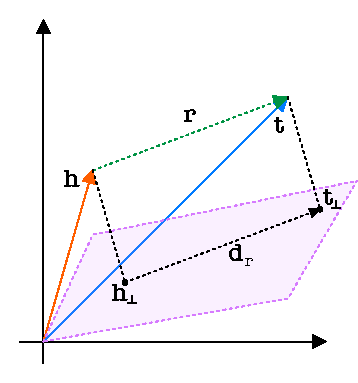
\includegraphics[width=0.5\textwidth]{figures/transh_illustration.pdf}
        \caption{A simple illustration of TransE} \label{transh-illustration}
\end{figure}
  

and similarly for the tail embedding \(\mathbf{t}\).

\begin{equation}
\mathbf{t}_{\perp}
  \;=\;
  \mathbf{t}
  \;-\;
  \bigl(\mathbf{w}_r^\top \mathbf{t}\bigr)\,\mathbf{w}_r
\end{equation}


The translation itself then takes place in this hyperplane:
\begin{equation}
    \mathbf{h}_\perp \;+\; \mathbf{d}_r \;\approx\; \mathbf{t}_\perp.
\end{equation}
  
This design allows different relations to transform entities in relation-specific ways, thus capturing more nuanced contextual behavior than TransE. During training, TransH typically also applies a \ac{MRL} approach similar to TransE. However, in this case the scoring function \(f(h, r, t)\) is the distance between \(\mathbf{h}_\perp + \mathbf{d}_r\) and \(\mathbf{t}_\perp\) (this work adopts the Euclidean distance or \(L_2\) norm),

\begin{equation}
  f(h, r, t)
  \;=\;
  \bigl\|
  \bigl(
    \mathbf{h}_{\perp}
    \;+\;
    \mathbf{d}_r
  \bigr)
  \;-\;
  \mathbf{t}_{\perp}
  \bigr\|_2,
\end{equation}
A lower value of \(f(h, r, t)\)
indicates a more plausible triple, since it implies that
\(\mathbf{h}_{\perp} + \mathbf{d}_r\)
is geometrically close to
\(\mathbf{t}_{\perp}\)
in the embedding space. By the end of training, TransH provides each entity in the \ac{BIM-KG} with a learned embedding, along with a normal vector and translation vector for each relation. These learned parameters enable a variety of link prediction tasks. For example, given \texttt{RoomA} $\xrightarrow{\text{isAdjascentTo}}$ \texttt{?}, the model can project \texttt{RoomA} onto the hyperplane for \texttt{isAdjacentTo}, apply the translation \(\mathbf{d}_{\texttt{isAdjacentTo}}\), and measure distances to all other entity embeddings to identify plausible neighbors. The main advantage of TransH over TransE in a BIM-KG setting is its capacity to handle varied semantics for the same entity depending on which relation it is involved in. Such flexibility is especially valuable if a single entity (such as a specific room or sensor) participates in multiple relationships that do not necessarily share the same geometric properties. However, it should be noted that TransH introduces additional parameters in the form of relation-specific normal vectors, which increases both the model’s expressiveness and its computational overhead. As a result, practitioners must weigh these factors against the potential gains in predictive accuracy and the need to handle more complex relation-specific behavior within \acp{BIM-KG}.
    \item
    \textbf{RotatE} represents entities and relations using complex-valued embeddings, where each dimension is treated as a point in the complex plane.
Concretely, for a triple \(\bigl(h, r, t\bigr)\), the head and tail entities \(h\) and \(t\) have embeddings
\(\mathbf{h}, \mathbf{t} \in \mathbb{C}^d\), while the relation \(r\) is associated with a vector
\(\mathbf{r} \in \mathbb{C}^d\). As illustrated in \autoref{fig:rotatE-illustration-1}, the key idea is to interpret each relation as a rotation in the complex plane, so that \(\mathbf{t}\) is obtained by rotating \(\mathbf{h}\) according to \(\mathbf{r}\).
In practice, this is realized via element-wise (Hadamard) multiplication:
\begin{equation}
  \mathbf{t} \;\approx\; \mathbf{h} \odot \mathbf{r},
\end{equation}

\begin{figure}[t]
    \centering
    \begin{subfigure}[t]{0.45\textwidth}
        \centering
        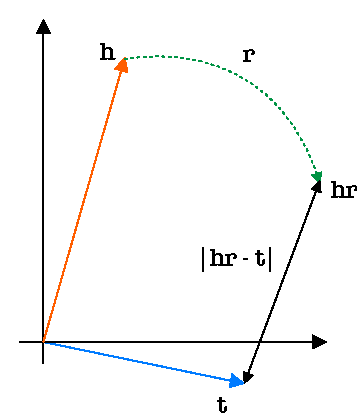
\includegraphics[width=\textwidth]{figures/rotate_illustration_1.pdf}
        \caption{A simple illustration of RotatE modeling \textbf{r} as a rotation in complex space}
        \label{fig:rotatE-illustration-1}
    \end{subfigure}
    \hfill
    \begin{subfigure}[t]{0.45\textwidth}
        \centering
        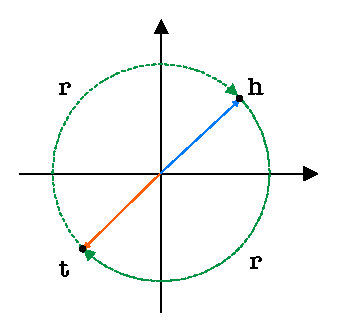
\includegraphics[width=\textwidth]{figures/rotate_illustration_2.pdf}
        \caption{An illustration of RotatE modeling symmetric relations \textbf{r}}
        \label{fig:rotatE-illustration-2}
    \end{subfigure}
    \caption{Simple illustration of RotatE's mechanics}
    \label{fig:rotatE-illustration}
\end{figure}
where every element of \(\mathbf{r}\) is constrained to have absolute value 1. This constraint
makes \(\mathbf{r}\) a pure phase vector that \emph{rotates} \(\mathbf{h}\) within each dimension
of \(\mathbb{C}^d\). By formulating relations as rotations, RotatE can naturally capture a variety of relational
patterns, including symmetry, antisymmetry, and inversion. For instance, a symmetric relation
like \(\texttt{isAdjacentTo}\) would imply that rotating \(\mathbf{h}\) by \(\mathbf{r}\) to arrive at
\(\mathbf{t}\) also means rotating \(\mathbf{t}\) by the same \(\mathbf{r}\) recovers \(\mathbf{h}\). This is illustrated in \autoref{fig:rotatE-illustration-2} . An antisymmetric relation would instead prohibit such a bidirectional mapping, as the same rotation
cannot be applied in reverse without changing the embedding position. In the context of a \ac{BIM-KG}, RotatE’s capacity to capture both symmetrical and asymmetrical relationships is particularly useful for encoding connections such as \(\texttt{isConnectedTo}\),
\(\texttt{isPartOf}\), or even hierarchical dependencies among building components (e.g., floors,
rooms, and sensors). Since \acp{BIM-KG} often mix functional, spatial, and compositional relationships, the flexibility offered by complex embeddings can lead to more accurate link predictions. Nonetheless, these potential benefits come at the expense of managing complex-valued vectors and additional hyperparameter tuning.


    \item
    \textbf{DistMult} is a bilinear embedding model that a simplification of RESCAL. In this model, both entities and relations are mapped to vectors
\(\mathbf{e}_i, \mathbf{r}_j \in \mathbb{R}^d\). Given a triple \(\bigl(h, r, t\bigr)\), DistMult employs
a scoring function based on element-wise (Hadamard) multiplication:
\begin{equation}
    f(h, r, t) 
  \;=\; 
  \mathbf{h}^\top 
  \bigl(\text{diag}\,\mathbf{r}\bigr)
  \,\mathbf{t}
  \;=\;
  \sum_{k=1}^d 
  h_k \,r_k \,t_k,
\end{equation}
  

where \(\mathbf{h}, \mathbf{t}, \mathbf{r}\) are the embeddings for the head entity \(h\), tail entity
\(t\), and relation \(r\), respectively, and \(\text{diag}\,\mathbf{r}\) denotes a diagonal matrix with
\(\mathbf{r}\) on its diagonal. Intuitively, DistMult captures relational influence by scaling each
dimension of \(\mathbf{h}\) by the corresponding dimension in \(\mathbf{r}\), which is then combined
with \(\mathbf{t}\). A notable property of DistMult is that it is inherently \emph{symmetric} with respect to
relations. That is, reversing the roles of head and tail does not change the score, since the
scoring function is commutative. This can be beneficial for knowledge graphs containing
primarily undirected or bidirectional relationships (such as \(\texttt{isAdjascentTo}\)) , but it becomes a limitation in scenarios
where antisymmetric or more complex relation patterns such as heirachical relationships (such as \(\texttt{hasProperty}\)) are prevalent. Still, for large-scale
building data requiring rapid inference, DistMult offers a favorable trade-off between speed
and performance, especially when combined with optimizations such as negative sampling and regularization. 

    \item
    \textbf{ComplEx} builds upon bilinear approaches such
as DistMult by allowing entity and relation embeddings to be complex-valued instead of being
restricted to real numbers. Specifically, each entity and relation \(e, r\) is mapped to a vector
\(\mathbf{e}, \mathbf{r} \in \mathbb{C}^d\). To score a triple \(\bigl(h, r, t\bigr)\), ComplEx applies
a bilinear form in the complex domain:
\[
  f(h, r, t)
  \;=\;
  \mathrm{Re}\Bigl(\bigl\langle \mathbf{h},\, \mathbf{r},\, \overline{\mathbf{t}} \bigr\rangle\Bigr)
  \;=\;
  \sum_{k=1}^d
  \bigl(h_k \;\cdot\; r_k \;\cdot\; \overline{t_k}\bigr),
\]
where \(\overline{t_k}\) denotes the complex conjugate of \(t_k\), and \(\mathrm{Re}(\cdot)\) takes
the real part of the resulting sum. By extending the entity and relation representations into the complex plane, ComplEx can model both symmetric and asymmetric relations, thus overcoming the inherent symmetry limitation of DistMult. For instance, when a relation is symmetric (such as \(\texttt{isAdjacentTo}\)), the imaginary parts of the embeddings cancel out in the scoring function, similarly to DistMult. Conversely,
when a relation is asymmetric, phase components in the complex embeddings can effectively capture directionality. The flexibility of handing both symmetric and asymmetric relations may lead to improved link prediction performance across a mix of relational patterns. However, as with other complex-valued models
like RotatE, ComplEx demands careful hyperparameter tuning (embedding dimension,learning rate, regularization) to ensure numerical stability and avoid overfitting. Its additional computational cost compared to real-valued approaches must be weighed against the potential accuracy gains when working with large-scale \ac{BIM-KG} datasets.


\end{enumerate}

\subsection{Datasets}
\label{subsec:experimental_datasets}
In these experiments, two publicly available \acp{BIM-KG} were used. These datasets are representative examples of how the Brick ontology\footnote{https://brickschema.org/} can be used to model real buildings - Rice Hall at University of Virginia \citep{Balaji2016Brick:Buildings} and Soda Hall at University of Carlifonia, Berkeley \citep{Balaji2016Brick:Buildings}, as detailed in \autoref{BIM-KG-datasets} - \autoref{tab:Soda Hall Facts} and shown in \autoref{fig:buildings_modeled_by_BRICK}. Brick is an open-source initiative aimed at standardizing the semantic descriptions of physical, logical, and virtual assets in buildings and their inter-relationships. An illustrative example of a building modeled using Brick is shown in \autoref{brick-building}. In this example, an \ac{AHU} supplies conditioned air to a \ac{VAV} Box, which adjusts the airflow to an \ac{HVAC} zone that has two rooms. The \ac{HVAC} zone has a thermostat equipped with a temperature and carbon dioxide sensor. Additionally, these two rooms are part of a lighting zone, and the lights in this zone are controlled by the building's lighting controller. The two datasets used in this thesis' experiments closely mirror this example building's setup, but on a larger scale. For an in-depth discussion on the creation and evaluation of these datasets, please refer to \cite{Balaji2016Brick:Buildings} and \cite{Balaji2018BrickApplications}.

\begin{figure}[t]
        \centering      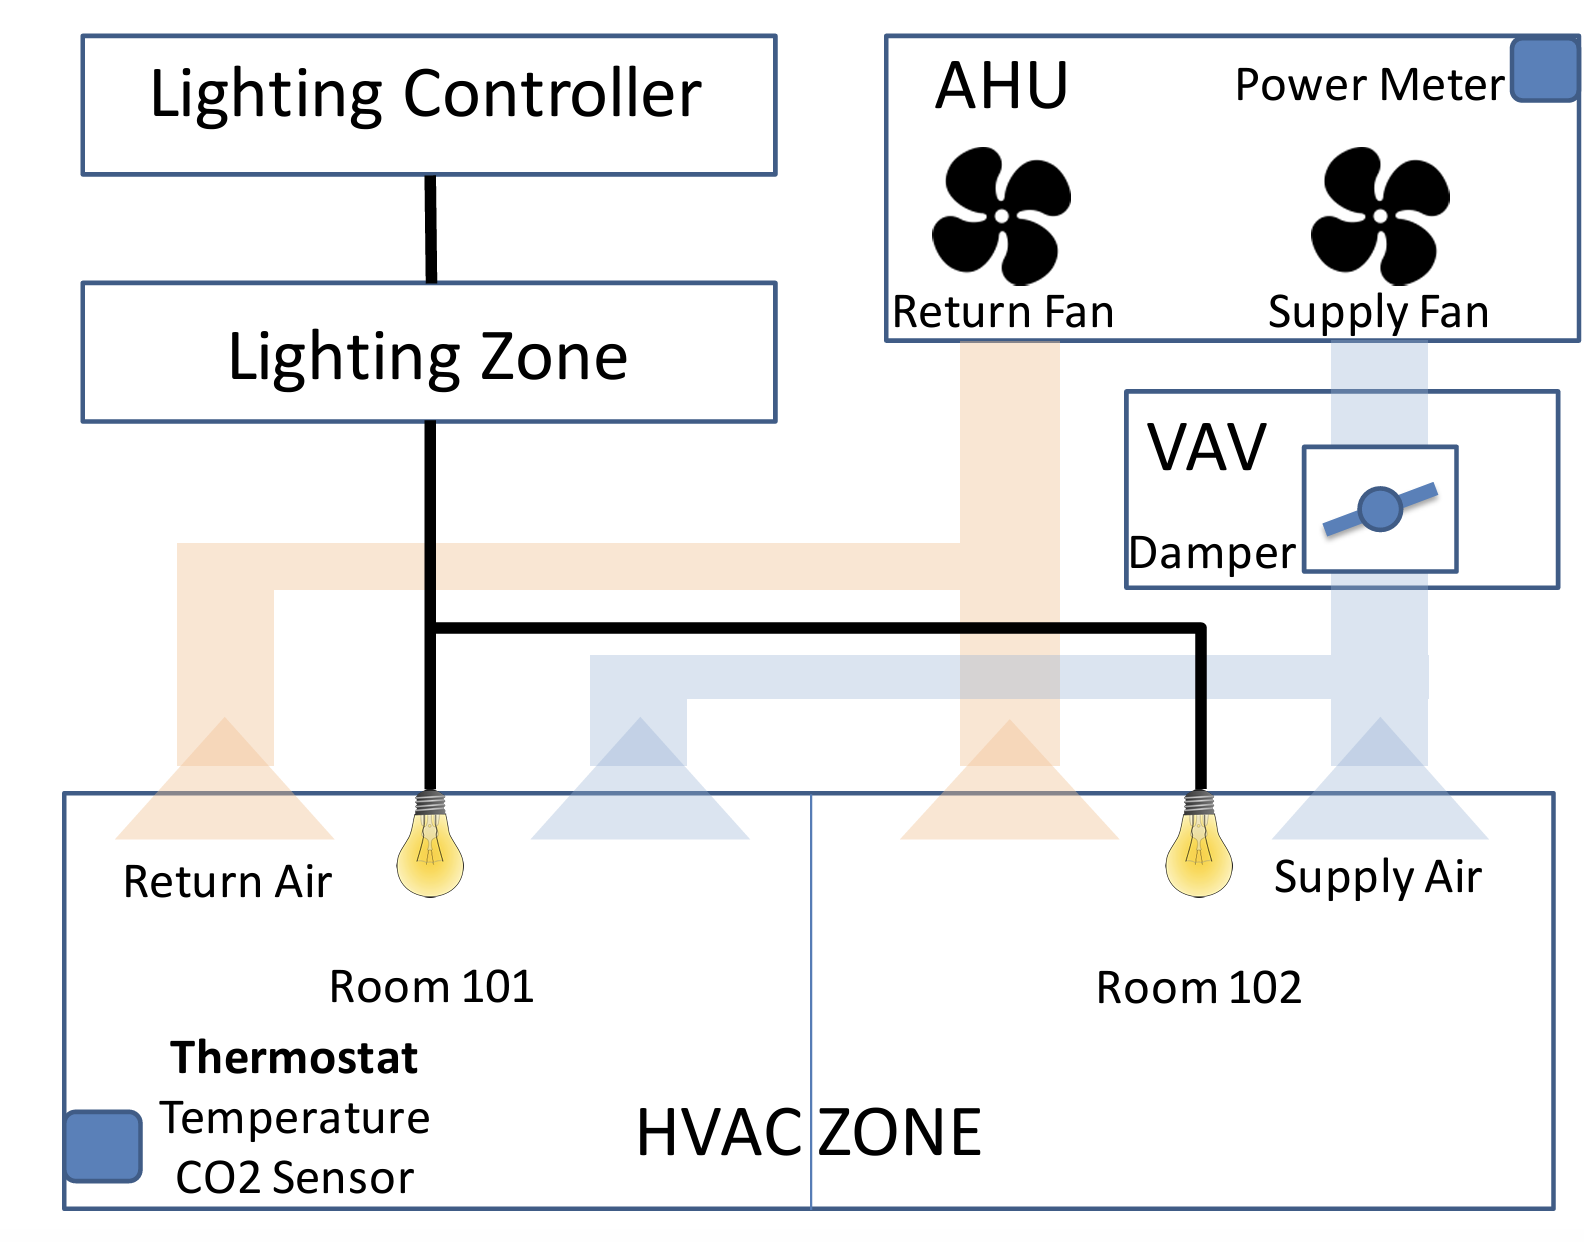
\includegraphics[width=0.5\textwidth]{figures/brick-building.png}
        \caption{A simple example highlighting the components of a building modeled by the Brick schema at a minimum. Source \citep{Balaji2016Brick:Buildings}} \label{brick-building}
\end{figure}

\begin{table}[!ht]
\centering
\caption{\ac{BIM-KG} datasets used in the performance analysis experiments}
\begin{tabular}{l|c|c|c|c}
\hline \hline \textbf{\ac{BIM-KG} Dataset} & \textbf{$|\mathcal{E}|$} & \textbf{$|\mathcal{K}|$} & \textbf{$\mathcal{E}$} Types & \textbf{$\mathcal{R}$} Types \bigstrut \\
\hline Rice Hall at University of Virginia & 810 & 1665 & 65 & 6 \\
Soda Hall at University of California, Berkeley & 1738 & 3774 & 36 & 9 \bigstrut \\
\hline
\end{tabular}
\label{BIM-KG-datasets}
\end{table}

\begin{table}[!ht]
    \centering
    \caption{Training dataset properties and structural patterns}
    \begin{tabular}{c|c|c|c}
    \hline \hline
        \textbf{Dataset} & \textbf{Density} & \textbf{Entity Heterogeneity} & \textbf{Average Degree} \bigstrut \\
        \hline
        Rice Hall & 0.002 & 65 & 3.664 \\
        
        Soda Hall & 0.001 & 36 & 4.342 \\
        \hline
    \end{tabular}
    \label{tab:BIM-KG-datasets_structural_patterns}
\end{table}

\begin{table}[!t]
\centering
\caption{Key Facts About Rice Hall, University of Virginia}
\label{tab:Rice Hall Facts}
\begin{tabular}{p{4cm}|p{10cm}}
\hline \hline
\textbf{Category}                & \textbf{Details}                                                                                  \bigstrut \\ \hline
Building                & Rice Hall, University of Virginia                                                                     \bigstrut  \\ \hline
Function                & Hosts the Computer Science Department                                                                \bigstrut   \\ \hline
Size                    & 100,000+ square feet                                                                                 \bigstrut   \\ \hline
Floors                  & 6                                                    \bigstrut   \\ \hline
Construction Year       & 2011\bigstrut    \\ \hline
Rooms                   & 120+ (faculty offices, teaching/research labs, study areas, conference rooms)                       \bigstrut    \\ \hline
\ac{BMS}      & Contracted with Trane\footnote{https://www.trane.com/}                                                                              \bigstrut    \\ \hline
HVAC System   & - 4 \acp{AHU} \newline - 30+ \acp{FCU} \newline - 120 \acp{VAV} 
\newline - Low-temperature chilled beams \newline - Ice tank-based chilling towers \newline - Enthalpy wheel heat recovery system \newline - Thermal storage system

            \bigstrut \\ \hline
Lighting System    & - Motorized shades \newline - Abundant daylight sensors \newline - Motion sensors                        \\ \hline
\end{tabular}
\bigskip

\caption{Key Facts About Soda Hall, UC Berkeley}
\label{tab:Soda Hall Facts}

\begin{tabular}{p{4cm}|p{10cm}}
\hline \hline
\textbf{Category}                & \textbf{Details}                                                                                     \bigstrut  \\ \hline
Building               & Soda Hall, UC Berkeley                                                                               \bigstrut   \\ \hline
Function                & Houses the Computer Science Department
\bigstrut   \\ \hline
Size                & 110,565+ square feet
\bigstrut    \\ \hline
Floors                  & 5                                                       \bigstrut   \\ \hline
Construction Year       & 1994\bigstrut    \\ \hline
Rooms                   & 200+ (small to medium-sized closed offices for faculty and graduate student groups)                       \bigstrut    \\ \hline
\acf{BMS} & Provided by the now-defunct Barrington Systems; exposes only \ac{HVAC} sensors                  \bigstrut    \\ \hline
\ac{HVAC} System              & - Pneumatic controls with 232 thermal zones. \newline - Periphery zones have \acp{VAV} with reheat \newline - Other zones without reheat. \newline - \acp{VAV} with reheat: Single control setpoint for both reheat and airflow using proprietary value mapping mechanism.  \newline - Contains redundant chillers, condensers, and cooling towers
\bigstrut   \\ \hline
\end{tabular}
\end{table}

\begin{figure}
    \centering
    \begin{subfigure}[b]{1\textwidth}
        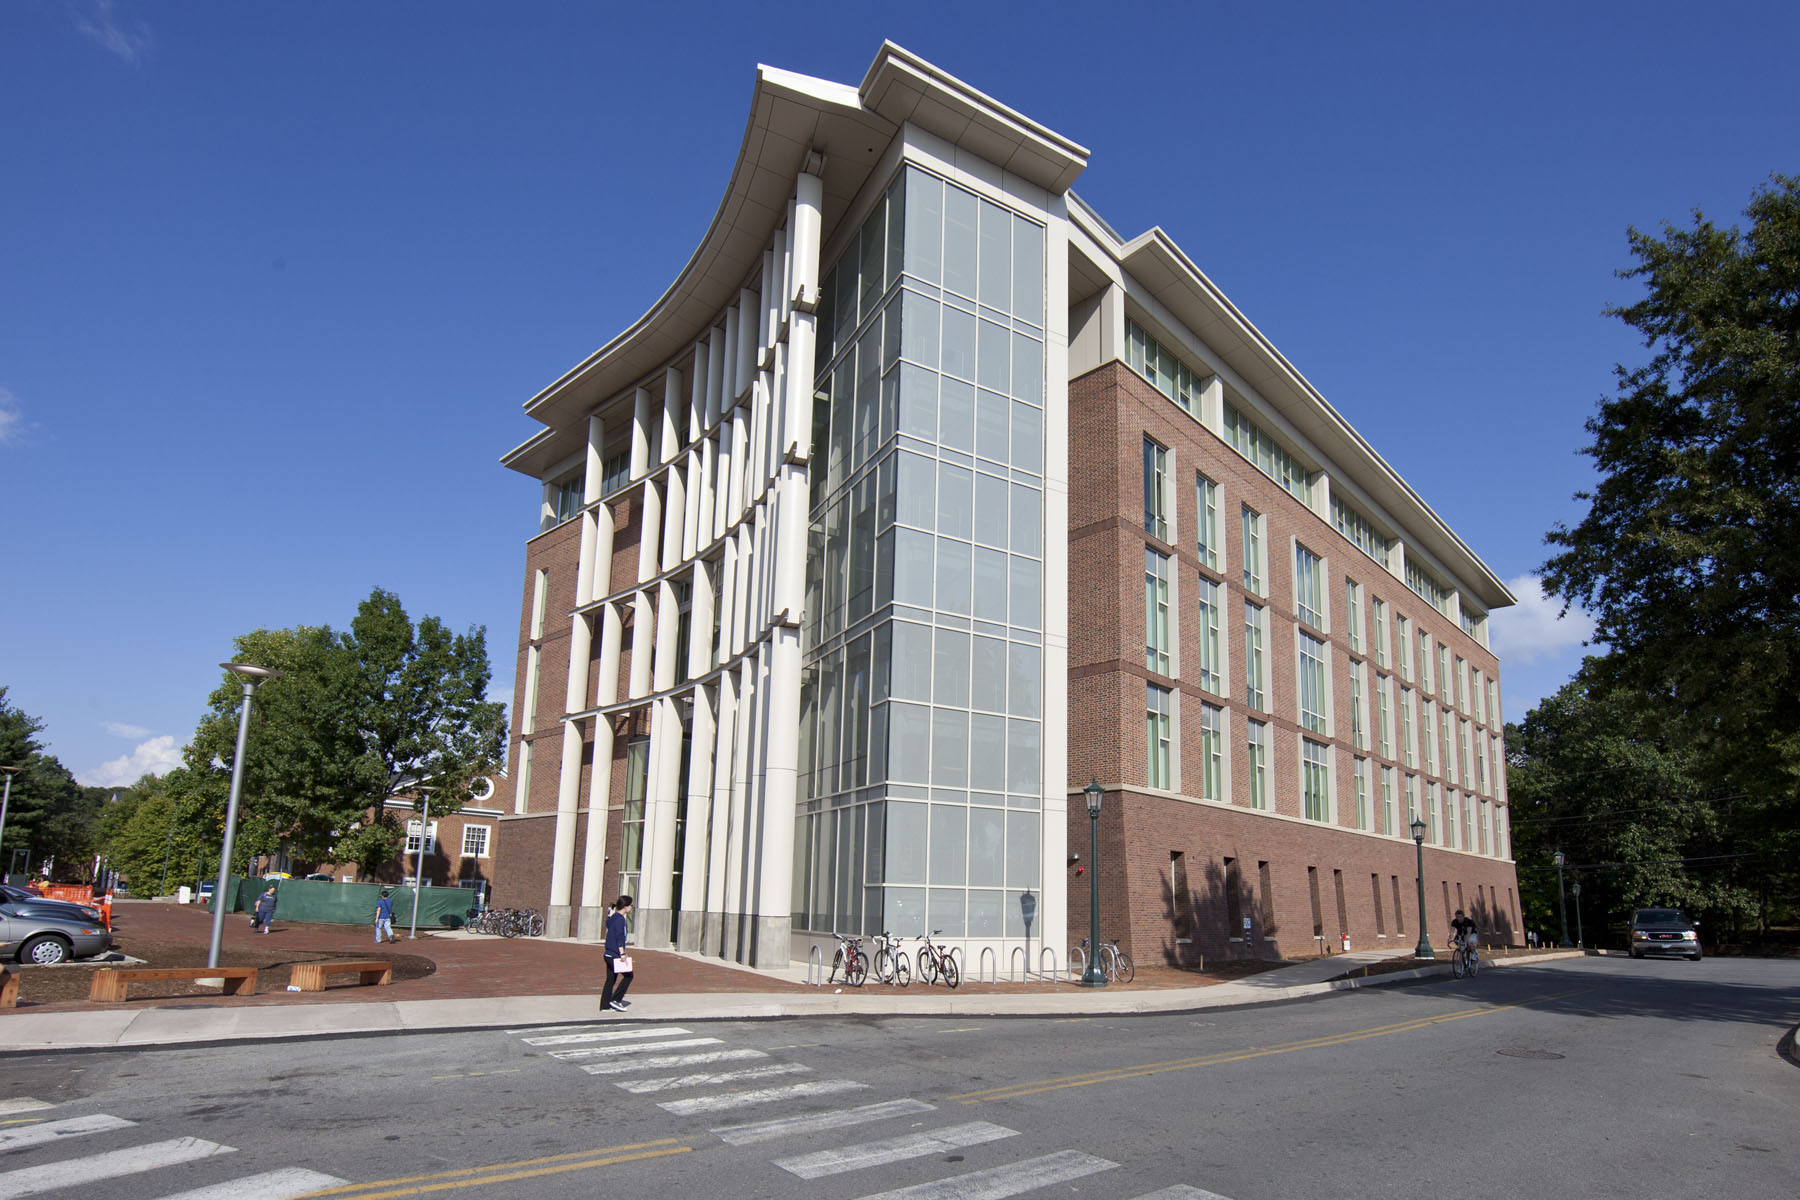
\includegraphics[width=\textwidth]{figures/rice_hall.jpg}
         \caption{Rice Hall at University of Virginia \newline (Source: \url{https://archello.com/project/university-of-virginia-rice-hall})}
        \label{subfig:rice_hall}
    \end{subfigure}
    % Spacing between subfigures. Adjust as needed.
    \hspace{0.05\textwidth}
    \begin{subfigure}[b]{1\textwidth}
        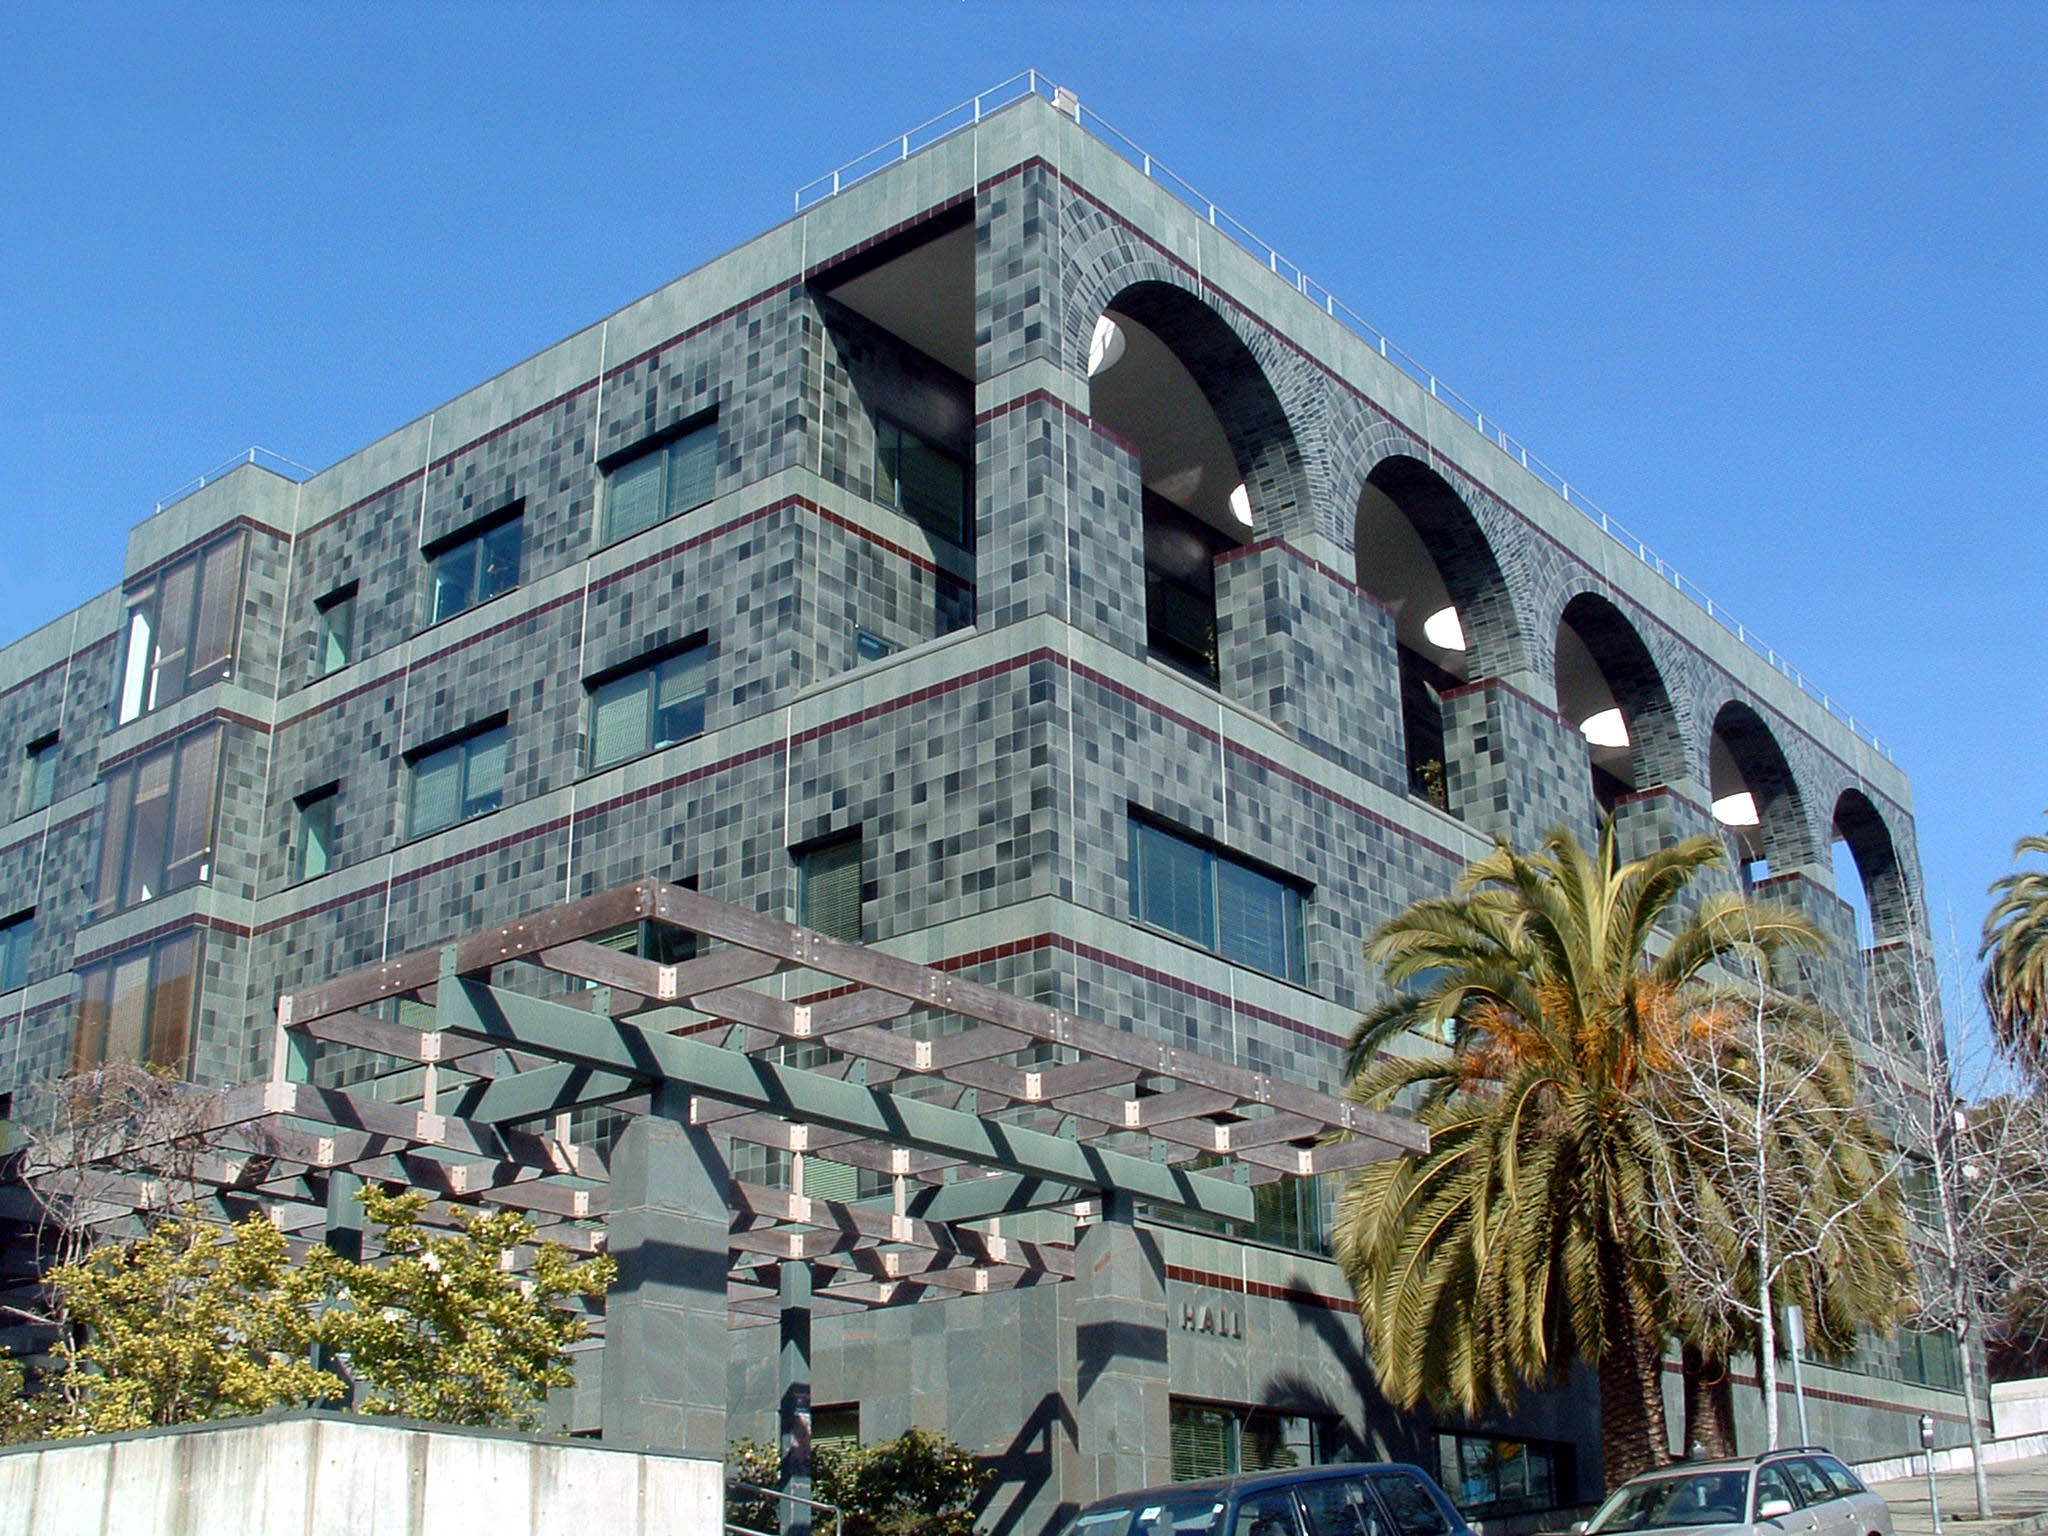
\includegraphics[width=\textwidth]{figures/Sodahall.jpeg}
        \caption{Soda Hall at University of California, Berkeley \newline (Source: \url{https://www.berkeley.edu/map/soda-hall/})}
               
        \label{subfig:soda_hall}
    \end{subfigure}
    \caption{The two buildings modelled by BRICK and adopted for this thesis' \ac{KRL} performance analysis experiments}
    \label{fig:buildings_modeled_by_BRICK}
\end{figure}

\subsection{Evaluation Protocol}
\label{subsec:evaluation_protocol}

The overarching goal of \ac{KRL} models is to learn entity and relation embeddings that capture the underlying structure and semantics of a knowledge graph. To learn reliable embeddings, a \ac{KRL} model needs to have the ability to distinguish between true facts and false facts in a knowledge graph. In reality, knowledge graphs are curated only with true facts yet both true and false facts are required for successful \ac{KRL} model training. When trained exclusively on true facts, a \ac{KRL} model never encounters invalid examples and thus risks learning a trivial strategy—namely, predicting every possible fact as true. By introducing corruption sets (i.e., negative samples generated by substituting entities in valid triples), the model is encouraged to discriminate between correct and incorrect facts. This process prevents the embeddings from collapsing into a single “\textit{always-true}” mode and enables more robust inference, particularly when dealing with missing or newly introduced facts in a \ac{BIM-KG}.  As mentioned earlier, in the \ac{OWA}, a fact cannot be considered false just because it does not exist in a knowledge graph however, when considering the \ac{LCWA}, a constrained variation of the \ac{CWA}, a knowledge graph is only locally complete i.e., if a fact \texttt{Room\_A} $\xrightarrow{\text{ssn:hasProperty}}$ \texttt{Temperature} is missing from a \ac{BIM-KG}, \ac{LCWA} interprets \texttt{Room A} as not having a Temperature property, but only within the context of this specific \ac{BIM-KG}. With this assumption, a set of negative triples $\mathcal{C}$ can be generated by altering either the head or tail entity of each triple \( (h, r, t) \) in a knowledge graph as shown in \autoref{eq:corruption} below;

\begin{equation}
\label{eq:corruption}
\mathcal{C} = \left\{(\hat{h}, r, t) \mid \hat{h} \in \mathcal{E}\right\} 
\cup \left\{(h, r, \hat{t}) \mid \hat{t} \in \mathcal{E}\right\}
\end{equation}

\noindent where \( \mathcal{E} \) is the set of all entities in the knowledge graph while \( \hat{h} \) and \( \hat{t} \) are the corrupted head and tail entities respectively. For any given triple \( (h, r, t) \) in the test set $\mathcal{K}_{\text{test}} \subseteq \mathcal{K}$, the left hand side of \autoref{eq:corruption}, $\left\{(\hat{h}, r, t) \mid \hat{h} \in \mathcal{E}\right\}$ corrupts the head entity \( h \) by replacing it with any other entity \( \hat{h} \) from the set \( \mathcal{E} \), creating triples of the form \( (\hat{h}, r, t) \) where \( \hat{h} \) is not the original head entity. Similarly $\left\{(h, r, \hat{t}) \mid \hat{t} \in \mathcal{E}\right\}$, corrupts the tail entity by replacing \( t \) with any other entity \(\hat{t} \in \mathcal{E}\), resulting in triples of the form \( (h, r, \hat{t}) \) where \( \hat{t} \) is not the original tail entity. To visualize this process better, consider a set of 5 entities \( \mathcal{E} = \{ \texttt{Space}, \texttt{Sensor}, \texttt{Site}, \texttt{Storey}, \texttt{Temperature} \} \) and a set of 2 relations \( \mathcal{R} = \{ \text{bot:hasElement}, \texttt{bot:adjascentElement} \} \). Given a triple, \texttt{Space} $\xrightarrow{\text{bot:hasElement}}$ \texttt{Sensor}, the corruption set \( \mathcal{C} \) below can be generated by replacing either the head or tail with entities from \( \mathcal{E} \). The first two rows hold corruptions where the tail has been replaced with \texttt{Site} and \texttt{Temperature}, respectively, while the last two rows hold corruptions where the head has been replaced with \texttt{Site} and \texttt{Storey}, respectively. 

\[
\mathcal{C} = 
\left[\begin{array}{ccc}

\textbf{Subject} & \textbf{Relation} & \textbf{Object} \\
\hline
\texttt{Space} & \texttt{bot:hasElement} & \texttt{Site} \\ 
\texttt{Space} & \texttt{bot:hasElement} & \texttt{Temperature} \\ 
\texttt{Site} & \texttt{bot:hasElement} & \texttt{Sensor} \\ 
\texttt{Storey} & \texttt{bot:hasElement} & \texttt{Sensor} \\ 
\end{array}\right]
\]

\noindent It is possible for some of the generated synthetic negatives to actually be true positives (already existing in $\mathcal{K}$). Whenever these are encountered in this work, they are removed from $\mathcal{K}$ using the filtered evaluation setting in \citep{Bordes2013} and \citep{Ali2020BringingFramework}, as their presence can skew the training results. 

\ac{KRL} treats link prediction as a \emph{learning-to-rank} problem. In this paradigm and for the rest of this thesis, a \emph{query} \( Q \) takes the form of a partially known triple such as \((h, r, ?)\), where the head entity \((h)\) and the relation \((r)\) are given, but the \emph{tail} \((?)\) is unknown. The model must then assign scores to a set of candidate tails, ranking the correct entity \emph{higher} than incorrect (or corrupted) alternatives. For instance, given a true triple \texttt{RoomA} $\xrightarrow{\text{ssn:hasProperty}}$ \texttt{Temperature} in a \ac{BIM-KG}, the query \texttt{RoomA} $\xrightarrow{\text{ssn:hasProperty}}$ \texttt{?} is answered by scoring every possible tail in the knowledge graph and ranking them. A well-trained model places \texttt{Temperature} near the top, while all corrupted versions---such as \texttt{RoomA} $\xrightarrow{\text{ssn:hasProperty}}$ \texttt{RoomB}---receive lower scores. The \emph{loss function} typically enforces this ranking objective. A common approach is a \emph{margin-based ranking loss}, where the model is penalized if a true triple's score is not sufficiently higher than its corresponding corrupted triple. Formally, for a true triple \(\bigl(h, r, t\bigr)\) and its corrupted counterpart \(\bigl(h', r, t'\bigr)\), the margin-based loss might look like:
\[
\mathcal{L} \;=\; \sum_{\substack{(h,r,t) \in \mathcal{P} \\ (h',r,t') \in \mathcal{C}}} \max\Bigl(0,\;\gamma \;+\; f\bigl(h',r,t'\bigr) \;-\; f\bigl(h,r,t\bigr)\Bigr),
\]
where \(f(\cdot)\) is the model's scoring function, \(\gamma\) is a margin, \(\mathcal{P}\) denotes the set of positive (true) triples, and \(\mathcal{C}\) the corrupted (negative) triples. This loss drives the model to \emph{rank} the true triple higher than any false candidate by a margin of \(\gamma\). Consequently, when evaluating on a holdout set \(\mathcal{K}_{\text{test}}\) , a well-performing model will \emph{score} (and thereby rank) the correct triple higher than any corrupted variation---leading to meaningful \acf{MR} or \acf{MRR} metrics that reflect the model's ability to discern true facts from false ones. When multiple triples in the test set, $\mathcal{K}_{\text{test}}$, receive the same score, this work resolves such ties by computing the \emph{mean} of the optimistic and pessimistic rankings. Concretely, in the \emph{optimistic} scenario, the true triple is assumed to occupy the \emph{top} position among all those with equal scores, whereas in the \emph{pessimistic} scenario, it is ranked \emph{last} among them. The final rank is the arithmetic mean of these two extremes, thereby providing a fair tie-break mechanism that avoids inflating or deflating the model’s performance metrics. Regarding performance metrics, as a starting point, this work adopts three commonly used ones namely; \acf{MRR}, Hits@K and \acf{AMR}. These are briefly defined below, however, for a more detailed narrative and discussion, reference is made to \citep{Ali2020BringingFramework}

\begin{enumerate}
    \item 
    \textbf{\ac{MRR}}: \ac{MRR} evaluates the effectiveness of information retrieval systems by calculating the average of the reciprocal ranks of the first relevant result for each query in a set of queries \( Q \). In simpler terms, for each query, you look at the rank position of the first correct answer, take the reciprocal of that rank, and then average those values across all queries. This provides a measure of how quickly the system finds the correct answer for queries. Mathematically, \ac{MRR} is defined as:
    
    \begin{equation}
    \label{eq:mrr}
    \text{MRR} = \frac{1}{|Q|} \sum_{i=1}^{|Q|} \frac{1}{\text{rank}_i}
    \end{equation}
    
    where \(\text{rank}_i\) is the rank of the true triple for the \(i\)-th query. For better intuition, imagine a \ac{BMS} that tries to answer some arbitrary building automation queries Q1, Q2 and Q3.

    \begin{enumerate}
        \item 
        Q1 = Which zone is \texttt{Room101} part of i.e., \texttt{Room101} $\xrightarrow{\text{isPartOf}}$ \texttt{?} ?

        \item 
        Q2 = Which zone does \texttt{HVAC1} serve i.e., \texttt{HVAC1} $\xrightarrow{\text{serves}}$ \texttt{?} ?

        \item 
        Q3 = Which system controls \texttt{Light1} i.e., \texttt{Light1} $\xrightarrow{\text{controlledBy}}$ \texttt{?} ?
        
    \end{enumerate}
    For each query, the \ac{BMS} makes three guesses with the first one being the one it thinks is most likely correct as shown in \autoref{tab:MRR-example} (the actual correct triple is marked with a \quad \checkmark). \ac{MRR} ranges from 0 to 1, with 1 indicating that all true triples are ranked first while 0 shows that none of the proposed results are correct. The \ac{MRR} for the \ac{BMS} is therefore calculated as $\frac{\frac{1}{3} + \frac{1}{2} + \frac{1}{2}}{3} \approx 0.44$ using \autoref{eq:mrr}
\begin{table}[]
    \centering
    \begin{tabular}{l|l|c|c}
    \hline \hline
    \textbf{Query} & \textbf{Proposed Results} & \textbf{Rank} & \textbf{Reciprocal Rank} \bigstrut \\
    \hline
    Q1 & 
    \begin{tabular}{@{}l@{}}
    \texttt{Room101} $\xrightarrow{\text{hasSensor}}$ \texttt{TempSensorA}, \\
    \texttt{Room101} $\xrightarrow{\text{isPartOf}}$ \texttt{BuildingB}, \\
    \textbf{\texttt{Room101} $\xrightarrow{\text{isPartOf}}$ \texttt{BuildingA}} \quad \checkmark
    \end{tabular} & 3 & $\frac{1}{3}$ \\
    \hline
    Q2 & 
    \begin{tabular}{@{}l@{}}
    \texttt{HVAC1} $\xrightarrow{\text{connectedTo}}$ \texttt{HVAC2}, \\
    \textbf{\texttt{HVAC1} $\xrightarrow{\text{serves}}$ \texttt{ZoneA}} \quad \checkmark, \\
    \texttt{HVAC1} $\xrightarrow{\text{hasPart}}$ \texttt{FanA} 
    \end{tabular} & 2 & $\frac{1}{2}$ \\
    \hline
    Q3 & 
    \begin{tabular}{@{}l@{}}
    \texttt{Light1} $\xrightarrow{\text{installedIn}}$ \texttt{Room101}, \\
    \textbf{\texttt{Light1} $\xrightarrow{\text{controlledBy}}$ \texttt{ControlSystemA}} \quad \checkmark, \\
    \texttt{Light1} $\xrightarrow{\text{hasSwitch}}$ \texttt{SwitchB}
    \end{tabular} & 2 & $\frac{1}{2}$ \\
    \hline
    \end{tabular}
    \caption{Ficticious reponses of an illustrative \ac{BMS} to 3 arbitrary queries and their reciprocal rank values. The correct response is marked with a \quad \checkmark}.
    \label{tab:MRR-example}
\end{table}

\item 
\textbf{Hits@\texttt{K}}: This metric measures the accuracy of a retrieval system by checking whether the correct answer is within the top \texttt{K} ranked results. Mathematically this is defined using the formula below

\begin{equation}
    \text{Hits@\texttt{K}} = \frac{1}{|Q|} \sum_{i=1}^{|Q|} \mathbf{1}(\text{rank}_i \leq \texttt{K})
\end{equation}

where \(\mathbf{1}(\text{rank}_i \leq K)\) is an indicator function that equals 1 if the true triple's rank is within the top \texttt{K}, and 0 otherwise. Hits@1, Hits@3, and Hits@10 are commonly used variations of this metric. Using the example in \autoref{tab:MRR-example}, hits@1 = $\frac{0}{3} = 0$, hits@3 = $\frac{3}{3} = 1$, hits@10 = $\frac{3}{3} = 1$ (the denominator for all being the 3 true existing facts, while the numerator is the number of correct facts appearing within the top \texttt{K}.  

\item 
\textbf{\ac{AMR}}: This metric complements \ac{MRR} and Hits@\texttt{K} metrics and has been shown to provide more fair comparisons between datasets of different sizes \citep{Berrendorf2020OnMethods}. Mathematically \ac{AMR} is defined in \autoref{eq:amr} as the ratio of the mean rank to its expected value;

\begin{equation}
\label{eq:amr}
\text{AMR} = \frac{\text{Mean Rank (MR)}}{\text{Expected Mean Rank (EMR)}}
\end{equation}

\end{enumerate}

\subsection{Implementation details}
All experiments were performed on a single Macbook Pro with an  Apple M1 Pro chip and 16GB RAM using PyKEEN \citep{Ali2020PyKEENEmbeddings}, a python-based library for \ac{KRL} built on top of PyTorch while hyperparameter optimizations were handled using Optuna \citep{Akiba2019Optuna:Framework}. The exact software versions are kept consistent and delineated in the source code attached to this thesis.